%%%%%%%%%%%%%%%%%%%%%%%%%%%%%%%%%%%%%%%%%%%%%%%%%%%%%%%%%%%%%%%%%%%%%
%
% 1.pdflatex main.tex 2.bibtex main.aux 3. pdflatex  main.tex 4. pdflatex  main.tex
%%%%%%%%%%%%%%%%%%%%%%%%%%%%%%%%%%%%%%%%%%%%%%%%%%%%%%%%%%%%%%%%%%%%%%

\documentclass[11pt]{article}
\usepackage{tabularx}
\newcolumntype{b}{X}
\newcolumntype{s}{>{\hsize=.5\hsize}X}
%\usepackage[spanish]{babel}
\usepackage[english]{babel}
%\usepackage[osf]{mathpazo}
%\usepackage{bookman}
\usepackage{palatino}
\usepackage[utf8]{inputenc}
\usepackage[utf8]{luainputenc}
%\usepackage{floatrow}

%\usepackage[T1]{fontenc}
%\usepackage{pgffor}
%\usepackage{lipsum}
%\usepackage[OT1]{fontenc}
\usepackage{graphicx}
\usepackage[export]{adjustbox} %frame in figure anovachi

\usepackage[a4paper]{geometry}
\usepackage[myheadings]{fullpage}
\usepackage{fancyhdr}
\usepackage{lastpage}
\usepackage{amsfonts, amsmath, amsthm, amssymb}
\theoremstyle{definition}
\newtheorem{definition}{Definition}[section]
 
\theoremstyle{remark}
\newtheorem*{remark}{Remark}
\DeclareMathOperator*{\argmax}{arg\,max}
\DeclareMathOperator*{\argmin}{arg\,min}
\usepackage{graphicx, wrapfig, subcaption, setspace, booktabs}
\usepackage[T1]{fontenc}
\usepackage[font=small, labelfont=bf]{caption}
\usepackage{fourier}
\usepackage{float}
%\usepackage[protrusion=true, expansion=true]{microtype}
%\usepackage[margin=1in]{geometry}
\usepackage{microtype}
\usepackage{sectsty}
\usepackage{url, lipsum}
\usepackage{listings}
\usepackage{xcolor}
\newcounter{countCode}
\newcommand{\HRule}[1]{\rule{\linewidth}{#1}}
\onehalfspacing
\setcounter{tocdepth}{5}
\setcounter{secnumdepth}{5}
\lstnewenvironment{code} [1][caption=Ponme caption, label=default]{%
\renewcommand*{\lstlistingname}{Python} 
  \setcounter{lstlisting}{\value{countCode}} 
  \lstset{ %
  language=python,
  basicstyle=\ttfamily\footnotesize,       % the size of the fonts that are used for the code
  numbers=left,                   % where to put the line-numbers
  numberstyle=\sc,      % the size of the fonts that are used for the line-numbers
  stepnumber=1,                   % the step between two line-numbers. 
  numbersep=5pt,                 % how far the line-numbers are from the code
  numberstyle=\color{red!50!blue},
    backgroundcolor=\color{lightgray!20},
  rulecolor=\color{blue},
  keywordstyle=\color{red}\bfseries,
  showspaces=false,               % show spaces adding particular underscores
  showstringspaces=false,         % underline spaces within strings
  showtabs=false,                 % show tabs within strings adding particular underscores
  frame=single,                   % adds a frame around the code
  framexleftmargin=0mm,
  numberblanklines=false,
  xleftmargin=5pt,
  breaklines=true,
  breakatwhitespace=true,
  breakautoindent=true,
  captionpos=t,
  texcl=true,
  tabsize=2,                      % sets default tabsize to 3 spaces
  extendedchars=true,
  inputencoding=utf8, 
  escapechar=\%,
  morekeywords={print, println, size, background, strokeWeight, fill, line, rect, ellipse, triangle, arc, save, PI, HALF_PI, QUARTER_PI, TAU, TWO_PI, width, height,},
  emph=[1]{print,println,}, emphstyle=[1]{\color{blue}}, % Mis palabras clave.
  emph=[2]{width,height,}, emphstyle=[2]{\bf\color{violet}}, % Mis palabras clave.
  emph=[3]{PI, HALF_PI, QUARTER_PI, TAU, TWO_PI}, emphstyle=[3]\color{orange!50!violet}, % Mis palabras clave.
  emph=[4]{line, rect, ellipse, triangle, arc,}, emphstyle=[4]\color{green!70!black}, % Mis palabras clave.
  %emph=[5]{size, background, strokeWeight, fill,}, emphstyle=[5]{\tt \color{red!30!blue}}, % Mis palabras clave.
  %emph={[2]sqrt,baset}, emphstyle={[2]\color{blue}}, % f(sqrt(2)), sqrt a nivel 2 se pondrá azul
#1}}{\addtocounter{countCode}{1}}
%-------------------------------------------------------------------------------
% HEADER & FOOTER
%-------------------------------------------------------------------------------
\pagestyle{fancy}
\fancyhf{}
\setlength\headheight{12pt}
\fancyhead[L]{Seven years of \emph{Proyecto Vallecas}}
\fancyhead[R]{Gómez-Ramírez et al. Fundaci\'on CIEN}
\fancyfoot[R]{\small{page} \thepage\ \small{of} \pageref{LastPage}}
%-------------------------------------------------------------------------------
% TITLE PAGE
%-------------------------------------------------------------------------------

\begin{document}
%IDENTIFICACIÓN DE FACTORES DE RIESGO EN DETERIORO COGNITIVO LEVE CON APRENDIZAJE AUTOMÁTICO: HACIA UNA AYUDA AL DIAGNÓSTICO MULTIFACTORIAL Y  AUTOINFORMADA

\title{ \normalsize \textsc{\emph{Proyecto Vallecas} Six years longitudinal study in healthy aging}
    \\ [2.0cm]
    \HRule{0.5pt} \\
    \LARGE \textbf{\uppercase{Exploratory Data Analysis in \emph{Proyecto Vallecas}: a six years longitudinal study in brain healthy aging}}
    \HRule{2pt} \\ [0.5cm]
    \normalsize \today \vspace*{5\baselineskip}}

\date{ }
%\author{
%    Jaime G\'omez-Ram\'irez, Marina \'Avila Villanueva, Bel\'en Frades Payo, Teodoro del Ser Quijano,\\ Meritxell Valent\'i Soler, María Ascensi\'on Zea Sevilla and Miguel \'Angel Fern\'andez-Bl\'azquez   \\  \\
%    \textbf{\large{Fundaci\'on Reina Sof\'ia}} \\
%    Centre for Research in Neurodegenarative Diseases
%    \\ \emph{Valderrebollo, 5, 28031 Madrid}
% }
\author{
    \textbf{\large{Big Data Research and Brain Analytics Unit}}   \\  \\
    \large{Fundaci\'on Reina Sof\'ia} \\
    Centre for Research in Neurodegenarative Diseases (Fundaci\'on CIEN)
    \\ \emph{Valderrebollo, 5, 28031 Madrid}
 }


\maketitle
\begin{center}

\includegraphics[width = 60mm]{figures/logo_mciu.png}
\end{center}
\newpage
\tableofcontents
\newpage

%-------------------------------------------------------------------------------
% Section title formatting
\sectionfont{\scshape}
%-------------------------------------------------------------------------------

%-------------------------------------------------------------------------------
% BODY

%CODE
%tensorflow/production/descriptive_stats.py
% eda_paper.py
%-------------------------------------------------------------------------------

\section*{Abstract}
Alzheimer's Disease (AD) is a complex, multifactorial and comorbid condition. The asymptomatic behavior in early stages of the disease is a paramount obstacle to formulate a preclinical and predictive model of AD. Not surprisingly, the AD drug approval rate is one of the lowest in the industry, an exiguous $0.4\%$. The identification of risk factors, preferably obtained by the subject herself, is sorely needed given that the incidence of Alzheimer’s disease grows exponentially with age \cite{ferri2005global}, \cite{ganguli2011age}. 

During the last 7 years, researchers at \emph{Proyecto Vallecas} have collected information about the project's volunteers, aged 70 or more. The \emph{Proyecto Vallecas} dataset includes information about a wide range of factors including magnetic resonance imaging, genetic, demographic, socioeconomic, cognitive performance, subjective memory complains, neuropsychiatric disorders, cardiovascular, sleep, diet, physical exercise and self assessed quality of life. The subjects in each visit were diagnosed as healthy, mild cognitive impairment (MCI) or dementia. 
%'CognitivePerformance', 'Diagnoses', 'Neuropsychiatric', 'QualityOfLife', 'Genetics_s', 'SCD', 'Demographics', 'Cardiovascular_s', 'PhysicalExercise_s', 'Sleep_s', 'Anthropometric_s', 'Diet_s', 'SocialEngagement_s', 'TraumaticBrainInjury_s', 'Demographics_s', 'EngagementExternalWorld_s'

In this study we perform Exploratory Data Analysis to summarize the main characteristics of this unique longitudinal dataset. The objective is to characterize the evolution of the collected features over time and most importantly, how their dynamics are related to cognitive decline. 
We identify time series characteristics with predictive power about cognitive decline. We show that the longitudinal dataset of \emph{Proyecto Vallecas}, if conveniently exploited, holds promise to identifying either factors promoting healthy aging and risk factors related to cognitive decline. 
 
\section{Introduction}
\label{se:int}
The Vallecas Project\footnote{We will use indistinctly \emph{Vallecas Project} and its vernacular \emph{Proyecto Vallecas}.} for early detection of AD is the most ambitious population-based study for healthy aging in Spain. The project is carried out at the Queen Sofia Foundation Alzheimer Center by a multidisciplinary team of researchers from the CIEN Foundation. The main objective of the Vallecas Project is to elucidate, through tracking of progression of the cohort, the best combination of features, clinical and others that are informative about developing cognitive impairment in the future. 
%Thus, it intends to identify a set of \emph{markers} to eventually determine the potential risk that an individual has to develop the disease in the future. 

The dataset at its inception in the first year contained 1,213 subjects who were studied using a large range of features. It is worth noting that the data set contains two types of observations: variables and time series. The former refers to variables that are measured only once, typically in the first year's visit (e.g. APOE genotyping or educational attainment) and the latter are variables with a time index attached (time series) measured at every subject's visit (e.g. results of cognitive performance tests, hippocampal volumetry, subjective memory complains etc.).
Importantly, the dimensionality of the dataset grows every year (new measurements of features are added) as it does the number of samples as the subjects keep coming for their yearly visits, however the number of examples collected per year decreases (some volunteers drop the study). 
Table \ref{tab:vallecasvars} shows the features types collected in The Vallecas Project.

\begin{table}
\begin{tabular}{ |p{4.4cm}|p{4.4cm}|p{4.4cm}| }
\hline
\hline
MRI & Genetics(APOE) & Demographics  \\
\hline
Anthropometric & Sleep & Quality of life \\
\hline
Cognitive performance & Subjective memory complains & Diet \\
\hline
Physical exercise & Diagnoses & Neuropsychiatric \\
\hline
Traumatic brain injury & Engagement external world &  \\
\hline

\hline
\end{tabular}
\caption{The table depicts a classification of the features of the \emph{Vallecas} dataset. Each item in the table refers to a cluster of features containing related features. For example, the weight and height of the participants are included under the term Anthropometric.
Note that some features are collected only during the first year for example APOE (\emph{Genetics}) or the education level (\emph{Demographics}), but for the most part, features are assessed at each year's visit.}
\label{tab:vallecasvars}
\end{table}

%%EDA paper1: Here we perform Exploratory Data Analysis (EDA). EDA is the first step in the data analysis process and is performed once the pre processing steps have finished. 
Figure \ref{fig:pv5years} depicts the number of volunteers for the seven years life of the project. The total number of visits collected so far is 4444. 

\begin{figure}[H]
        \centering
        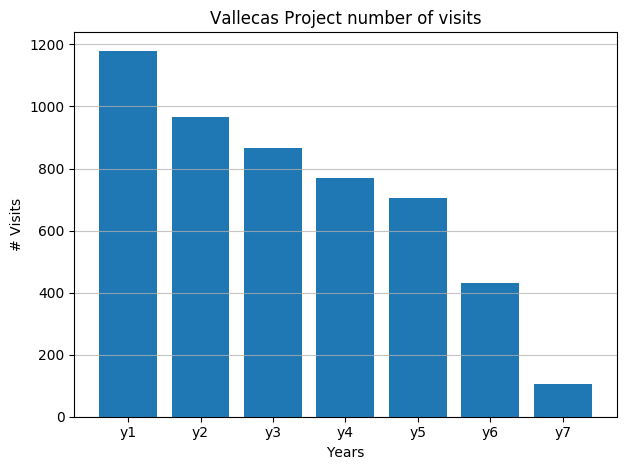
\includegraphics[keepaspectratio, width=0.6\linewidth]{figures/Fig_visits}
        \caption{Number of volunteers across seven years of \emph{Proyecto Vallecas}. As expected, the number of subjects decreases across time. The number of subjects in the year 1 was 1213 of which 33 were removed because were diagnosed with MCI or AD resulting in 1180 subjects recruited to participate in the study in year 1. 965 of the initial 1180 came for a second visit ($18\%$ drop rate), 865 in year 3 ($27\%$ drop rate from year 1), 770 in year 4 ($35\%$ drop rate from year 1), 704 in year 5 ($40\%$ drop rate from year 1), 491 in year 6($58\%$ drop rate from year 1) and 195 in year 7 which at this moment still ongoing. The total number of visits in five years amounts to 5203.} \label{fig:pv5years}
\end{figure}

%The structure of the document is as follows. Section \ref{se:eda} provides a comprehensive description of the information collected, the description relies upon visual charts and we also study the distribution of some key features collected in \emph{Proyecto Vallecas} dataset.
%Section \ref{se:met} shows statistical tests and the correlation analysis paying special attention to the evolution of the longitudinal variables and their underlying relationship with cognitive performance. 
%This section describes the features that are most strongly related to cognitive decline for both static (measured once) and dynamic variables (measured every year). We extract features from the longitudinal features to build a classifier based on relevant features extracted from time series \cite{christ2018time}. We conclude with the discussion of the results and future works in Section \ref{se:con} connecting our findings with previous populational studies.  

\section{Exploratory Data Analysis static variables}
\label{sse:eda}
%Static as the correlate with conversion
In this section we perform Exploratory Data Analysis (EDA). The objective of EDA is to build graphical representations that help us make sense of the data. EDA gives us a bird's eye of the dataset aiding at identifying patterns and trends and most importantly, assisting in framing the type of questions we want to ask.
EDA relies upon a careful pre-processing of the dataset. We perform EDA in a succession of steps. We will start with a preliminary data analysis plotting basic information of the dataset such as the age distribution and other demographics of the participants. 
We will also study the distribution of the most significant features of all type of features indicated in Table \ref{tab:vallecasvars}. Furthermore, we plot the distribution of cognitive decline conditional to other features. This will set the stage for the correlation analysis described in Section \ref{se:res} for both static (one observation) and dynamic variables (time series).
%YS cambio, now i know i want to do, write this when all done


% features_dict['Anthropometric_s'] == ['lat_manual', 'pabd', 'peso', 'talla', 'audi', 'visu', 'imc']
% Plot 'pabd', 'peso', 'talla', 'audi'
\subsection{Genetic, Anthropometric and Demographic}
\label{ssse:ant}

% features_dict['Demographics_s'] == ['edad', 'edad_visita7']
The major risk of developing AD is age. Figure \ref{fig:ages} shows the age of the participants at the inception of the project and the age of the participants that came to their sixth visit.

\begin{figure}[H]
        \centering
        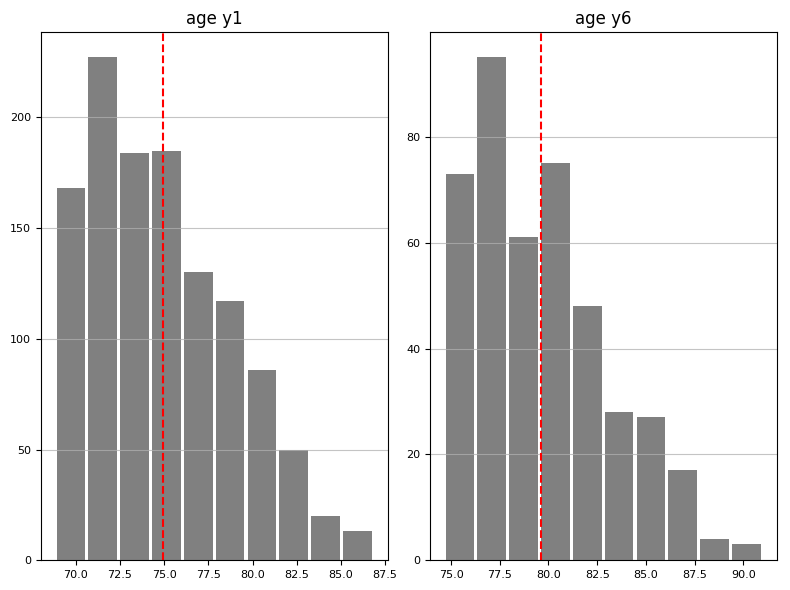
\includegraphics[keepaspectratio, width=.6\linewidth]{figures/Fig_ages}
        \caption{Histogram of the age of the participants in the first and last years of the \emph{Proyecto Vallecas} dataset. The youngest and the oldest participant in year 1 were 69 and 86 years old respectively. In year 6, the minimum and maximum ages were 76 and 89 respectively.} 
        \label{fig:ages}
\end{figure}

%Amyloid beta ($A\beta$) plaques is one of the two hallmarks of AD, the other is tau neurofibrillary tangles
Human apolipoprotein $\3epsilon$ (APO$\epsilon$) is a cholesterol carrier that supports lipid transport protein coded by the polymorphic APOE gene. The APOE gene has three major alleles: $\epsilon2$, $\epsilon3$ and $\epsilon4$ \cite{mahley2000apolipoprotein}, \cite{hauser2011apolipoprotein}. The presence of the $\epsilon4$ allele is thought to be one of the major risk factor for developing sporadic AD. Carriers of one copy of the  $\epsilon4$ allele (heterozygotes) have an increased risk of 3-4 times of developing sporadic AD, and carriers of two copies of the $\epsilon4$ allele (homozygotes) have an increased risk of 8-12 times of developing the disease \cite{heffernan2016neurobiology}. 

The APO$\epsilon4$ variant is the largest known genetic risk factor for late-onset sporadic Alzheimer's disease (AD). This risk, however, varies by demographic factors such as sex and ethnicity. For instance, Nigerian blacks have the highest observed frequency of the APO$\epsilon4$ allele in world populations, but at the same time AD is apparently less frequent in Nigerians than in other populations \cite{sepehrnia1989genetic}.

The estimated worldwide human allele frequencies of the APO$\epsilon4$ allele in the normal population is between $10-15\%$\cite{myers1996apolipoprotein} ($13.7\%$ for "Caucasian"\footnote{We use the term "Caucasian" as it is used in the referred work, however this labeling can be meaningless due to the large heterogeneity and non specificity in the population that the label is supposed to name \cite{bhopal1998white}} populations \cite{corder1994protective}). 
%APOE allele frequencies were: e2, 8.3%; e3, 78%; e4, 13.7% comparable to those reported for Caucasian populations (Corder et al., 1994
On the other hand, $40–65\%$ of subjects diagnosed with AD have one or two copies of the $APO\epsilon4$ allele \cite{saunders1993association}. 
%But why would such a seemingly deleterious allele survive in the population?

Figure \ref{fig:apoe} shows the APOE Genotyping in \emph{The Vallecas Project}, classifying the subjects in three groups depending on whether they lack any copy of the APO$\epsilon4$ allele, have one copy of APO$\epsilon4$ (heterozygotes) or have two copies of APO$\epsilon4$ (homozygotes) \cite{farrer1997effects}. In this cohort, $82\%$ were APO$\epsilon4$ negative, $17\%$ APO$\epsilon4$ heterozygotes and $1\%$ APO$\epsilon4$ homozygotes. 
%DO p(AD|+ in apoe)

\begin{figure}[H]
        \centering
        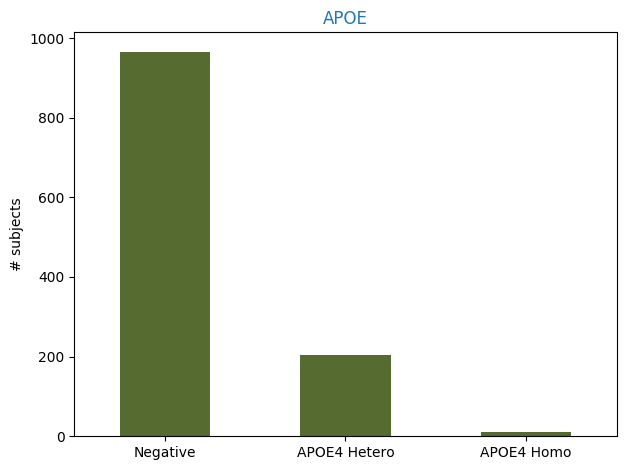
\includegraphics[keepaspectratio, width=0.6\linewidth]{figures/Fig_apoe}
        \caption{APOE Genotyping testing in \emph{Proyecto Vallecas} dataset. $17\%$ of subjects carry at least one copy of the $\epsilon4$, slightly higher than the worldwide estimates in Caucasian population ($13.7\%$) \cite{farrer1997effects}} 
        \label{fig:apoe}
\end{figure}

% \colorbox{yellow}{Black text on red background}
% \fcolorbox{blue}{red}%
%   {Black text, red  dbackground, blue frame} d
% \fbox{\begin{minipage}{40em}
% \begin{center}
% The quick brown fox jumps right over the lazy dog. the quick brown fox 
%   jumps right over the lazy dog. the quick brown fox jumps right over the lazy 
%   dog. the quick brown fox jumps right over the lazy dog. the quick brown fox 
%   jumps right over the lazy dog. the quick brown fox jumps right over the lazy 
%   dog. the quick brown fox jumps right over the lazy dog. the quick brown fox 
%   jumps right over the lazy dog.
% \end{center}
% \end{minipage}}

People with a higher body mass index (BMI) in midlife are more likely to develop dementia. This conclusion was achieved in a study that pooled BMI data from a total of 1.3 million subjects in a period of up to 38 years from the original measurement of their BMI \cite{kivimaki2018body}. 
The relationship between MBI and developing dementia is however complicated, the study found that people who developed dementia tend to have a lower than average BMI in the years leading up to the diagnosis. 
Nevertheless, the causal link between BMI and dementia is debatable, the reported relationship between BMI and dementia could be a product of the early stages of the disease rather than a risk factor. 

Any causal statement relies upon the occurrence of events in time and since the onset of dementia is unknown, we must be very cautious about establishing causal links between, in this case, BMI and the diagnosis of AD.   
%Higher midlife body mass index (BMI) is suggested to increase the risk of dementia, but weight loss during the preclinical dementia phase may mask such effects.
We must thus keep in mind the caveat that while higher BMI in midlife (our sample is composed of elder subjects) 
could be a risk factor for dementia, preclinical (undetected) stages of the disease could also produce weight loss and mask this effect. 

Figure \ref{fig:anthro} shows the distribution of anthropometric variables: BMI, abdominal perimeter, weight and height, measured in the first visit. 
%BMI is calculated by dividing your weight in kilograms by your height in meters squared. 
%https://www.alzheimersresearchuk.org/high-bmi-linked-increased-risk-dementia-later-life/
According to the BMI metrics ($25.0—29.9$ overweight, $>30.0$ obese) our population is overweight (right tail is longer than left tail in the top left histogram. Obesity (Higher midlife BMI) is related to higher risk of dementia and AD, independently of obesity-related risk factors and co-morbidities \cite{tolppanen2014midlife}, \cite{nepal2014rising}. However, a recent meta-analysis \cite{winter2014bmi} found not association between overweight and an increased risk of mortality, on the other hand, the study found an increased risk for those at the lower end (BMI $< 23.0$). If we pay attention to this results, weight loss is an useful feature to monitor in older age.

%CODE
%dataframe['imc'].skew(). pd.qcut(dataframe['imc'],4)
\begin{figure}[H]
        \centering
        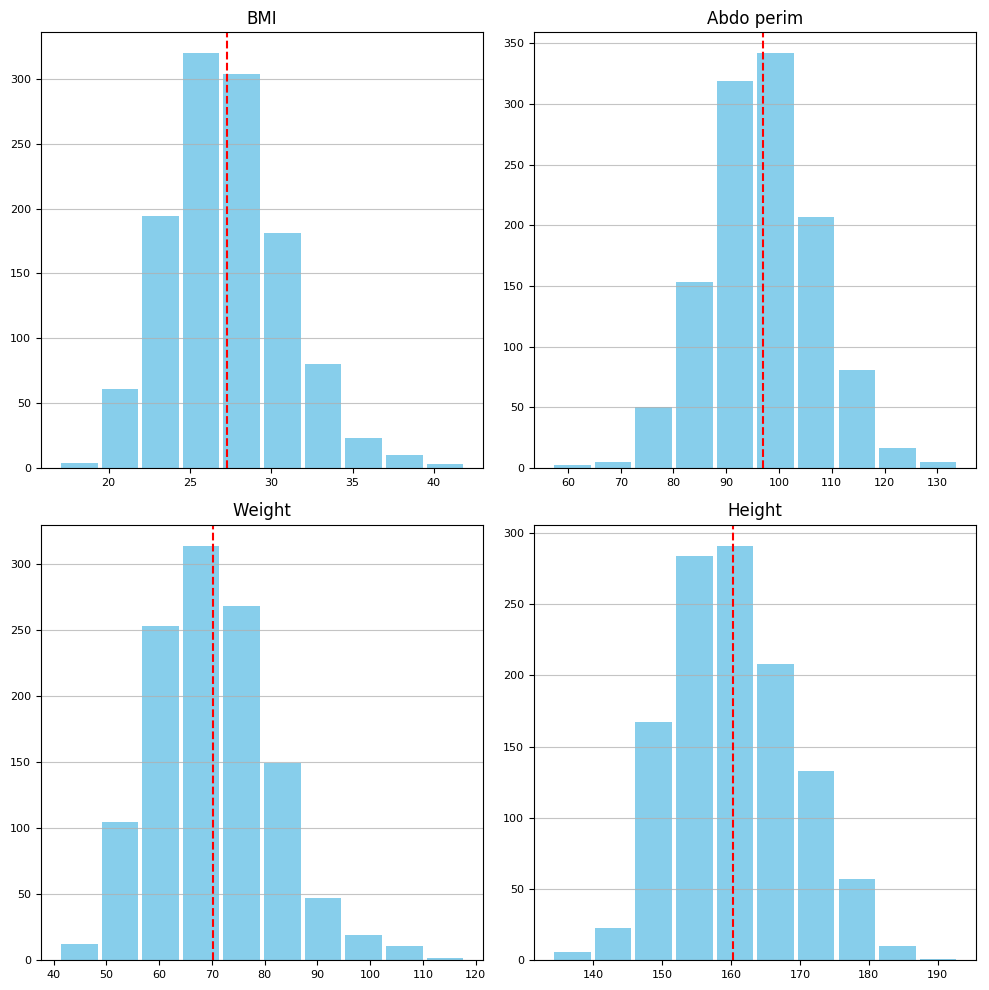
\includegraphics[keepaspectratio, width=.8\linewidth]{figures/Fig_anthro}
        \caption{Histogram of anthropometric variables measured in year 1 of \emph{Proyecto Vallecas} dataset. Clockwise, Body Mass Index (min=16.95, max=41.93), abdominal perimeter (min=57cm, max=134cm), weight (min=41kg, max=118kg) and height (min=134cm, max=193cm). 
        The mean and standard deviation of the BMI in our population is $\mu_{BMI}=27.3$ and $\sigma_{BMI}=3.6$. $26.8\%$ of the population have a healthy weight ($BMI \in [18.5, 25]$), $51.8\%$ have over weight ($BMI \in [25,30]$) and $21.4\%$ are obese ($BMI > 30$). 
        Skewness, a measure of the asymmetry of the probability distribution, in BMI, weight and height is positive (0.37,0.49, 0.29).} 
        \label{fig:anthro}
\end{figure}

Although there are gender-specific risk factors for AD a convincing account of how brain structure and function  may vary by sex is missing \cite{mielke2014clinical}. Epidemiological studies show that after age, the main risk factor for developing AD  is sex \cite{vina2010women}, \cite{mazure2016sex}. While it is well known that the incidence of the disease is higher in women, it is far from clear that this can be entirely attributed to the higher longevity of women versus men. 

Mitochondria of younger women are better protected against amyloid-beta toxicity, but this advantage lessens with age. Estrogenic therapies to deal with mitochondrial damage in AD have failed so far. A 2014 cohort study reports that women with the APO$\epsilon4$ allele are at greater risk of developing AD than are men with this allele \cite{altmann2014sex}. The same study argues that the inconsistency of previous findings about this allele could be motivated by researchers overlooking the APO$\epsilon4$-sex interaction.

Women and men seem to have different clinical presentations, according to \cite{sinforiani2010impact} men tend to show more aggressive behaviours and more comorbidity, while women would present more affective symptoms and disability but longer survival times. These behavioral differences would indicate sex-based neuropathologies in need of clarification. A report from the MIRIAD dataset \cite{malone2013miriad} -a database of volumetric MRI brain-scans of Alzheimer's sufferers and healthy elderly people- suggest that hippocampal atrophy in subjects with patients with probable AD has a faster rate in women as compared to men, making female sex a risk factor for faster descent into AD \cite{ardekani2016analysis}.

%laterality
%https://www.awakeningfromalzheimers.com/what-being-right-or-left-handed-says-about-alzheimers-risk/
$6.2\%$ of \emph{The Vallecas Project} cohort is not right-handed. A 1986 study reported that compared to right handers, left handers are less vulnerable to the cognitive problems associated with AD \cite{de1986reduced}. However, hand laterality seems play a very marginal role, if any, in AD. In fact, research relating handedness preference and memory function have been abandoned since the early pre-MRI years. Figure \ref{fig:sexlat} shows the histogram for sex and hand laterality in the \emph{Vallecas} cohort.
%Change this figure
\begin{figure}[H]
        \centering
        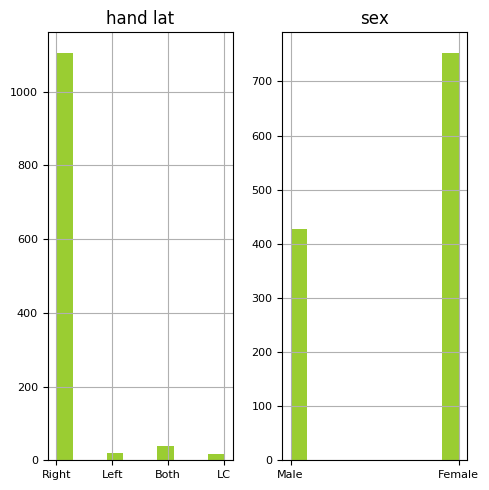
\includegraphics[keepaspectratio, width=.6\linewidth]{figures/Fig_sexlat}
        \caption{Histogram of hand laterality (left) and sex (right). There is majority of females, 753 versus 427 males. The right handed are 1106, left 19, ambidextrous 39 and 16 were forced right about born left,  $6.2\%$ of non-right-handers versus $93.8\%$ of right-handers.} 
        \label{fig:sexlat}
\end{figure}

A 2018 study using data data on cognition from the 2000 and 2010 Health and Retirement Study \cite{crimmins2018educational}, found that people with more education have lower prevalence of dementia and more years of cognitively healthy life. In a postmortem study of 86 brains, researchers found an associations between number of children and neuropathology of AD for women only \cite{beeri2009number}. Researchers argue that this difference may be due to sex-specific mechanisms (e.g. estrogen) rather socio economic differences present in both men and women. However, in addition to the limitations of the study (women were older than men) the ways in which motherhood affect AD risk are more complex, even producing inconsistent results. A 3.5 thousands women study \cite{jang2018differential} found that women who give birth to five or more children may be more likely to develop Alzheimer's disease than women who have fewer births, furthermore, incomplete pregnancy was associated with lower risk of AD in late life. But in a study with 14.5 thousands women presented at the 2018 Alzheimer’s Association International Conference in Chicago, researchers reported that women with three or more children had a 12 percent lower risk of dementia compared to women with one child \cite{AAIC2018}.

Social isolation and loneliness is believed to be a risk factor in AD (\cite{holmen1992loneliness}, \cite{fratiglioni2000influence}, \cite{shankar2013social}, \cite{holwerda2014feelings}, \cite{evans2018social}). A 2007 longitudinal study with up to 4 years of in-home follow up, reported a positive association between loneliness and an increased risk of late-life dementia \cite{wilson2007loneliness}. 

Figure \ref{fig:demo} depicts demographic variables including: educational attainment, number of sons, years of work as an employee, self-assessed economic status, marital status and the number of people living at home.
\begin{figure}[H]
        \centering
        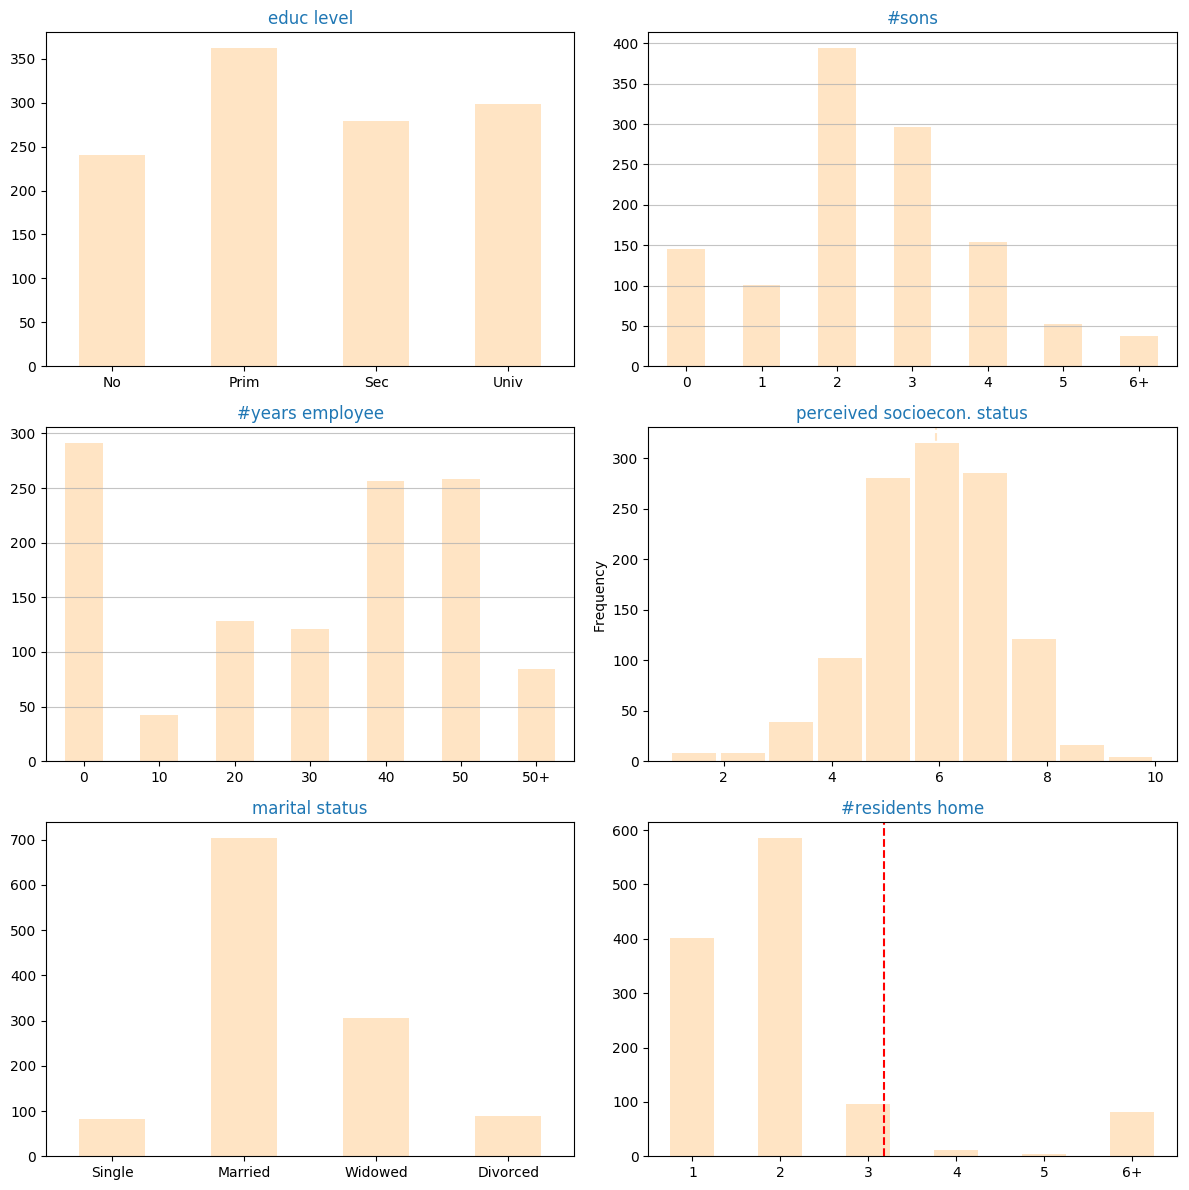
\includegraphics[keepaspectratio, width=\linewidth]{figures/Fig_demo}
        \caption{Histogram of demographic variables in the \emph{Proyecto Vallecas} dataset measured in the first year. Clockwise, educational attainment classified as \emph{no formal education, primary school, secondary school and university degree}, number of sons, number of years of work as an employee, self-assessed economic status (1 the lowest, 10 the highest, marital status (\emph{single, married, widows, divorced}) and the number of people living at home.} 
        \label{fig:demo}
\end{figure}

%['renta', 'nivelrenta', 'educrenta', 'municipio', 'barrio', 'distrito', 'sexo', 'nivel_educativo', 'anos_escolaridad', 'familial_ad', 'sdestciv', 'sdhijos', 'numhij', 'sdvive', 'sdocupac', 'sdresid', 'sdtrabaja', 'sdeconom', 'sdatrb']
We close the section of demographic variables with census income estimate based on the ZIP code. Lifestyle factors affect the susceptibility to developing AD and these factors are in many ways related to the level of personal income. \emph{Ceteris paribus}, higher income subjects have better opportunities for education, rich and varied diet, leisure and health-care facilities than residents of lower income areas. The influence of the income level on AD mortality is, however, uncertain. Nevertheless, the variation of income-related modifiable lifestyle risk factors (diet, physical exercise, social life, job) across life span, makes it very difficult if not impossible to suggest a clear association between income level and risk of developing dementia \cite{stkepkowski2015correlation}, \cite{ferri2017dementia}.

Stress is a coping mechanism for taxing changes impinged upon us in our environment. In particular, allostasis is the adaptive mechanism put in place by the body in anticipation for departures from homeostatic equilibrium triggered by stressful situations \cite{ellis2014beyond}. However, not all the stressors are detrimental, stressors can also have beneficial effects. 
The duration and cyclicity of the stress is particularly important and chronic stress is unequivocally detrimental. The accumulative impact of neuroendocrine responses to chronic stressors might impair homeoastic mechanisms, setting the basis for depression, neurodegenerative disorders and other pathogenic conditions \cite{bisht2018chronic}. Financially stressed individuals with recurrent difficulties to making ends meet, suffer from psychological stress that in turn may lead to cellular damage due to inflammation and oxidative damage \cite{hayashi2015conversion}. 

Figure \ref{fig:incomeresidency} shows the income distribution of the subjects estimated based on their home residency. 

%A more in detail representation of the home residency is shown in figure \ref{fig:resid_detail}

\begin{figure}[H]
        \centering
        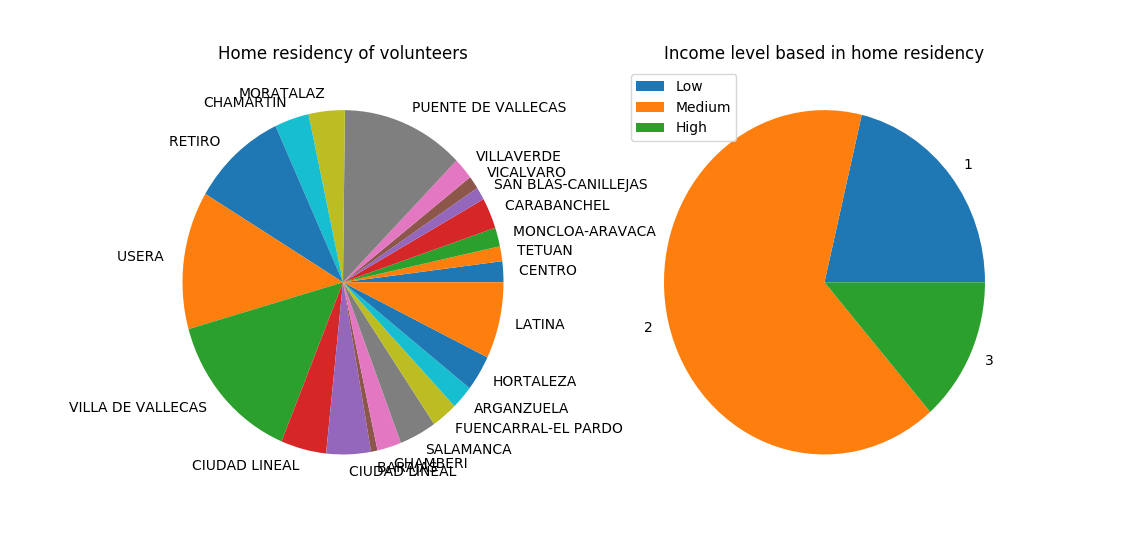
\includegraphics[keepaspectratio, width=\linewidth]{figures/incomeresidency}
        \caption{On the left, distribution of home residency by districts of \emph{Proyecto Vallecas} volunteers. All districts of the city of Madrid are represented. Note that there are 156 subjects of a total of 1180 that are not residents in the city of Madrid and are not included here. On the right, we plot the income distribution as estimated based on the home residency, 251 subjects live in low income areas, 769 in medium income areas and 160 in high income neighborhoods of Madrid.
        } \label{fig:incomeresidency}
\end{figure}

% Create figure and dsave it properly as png
% \begin{figure}[]
%         \centering
%         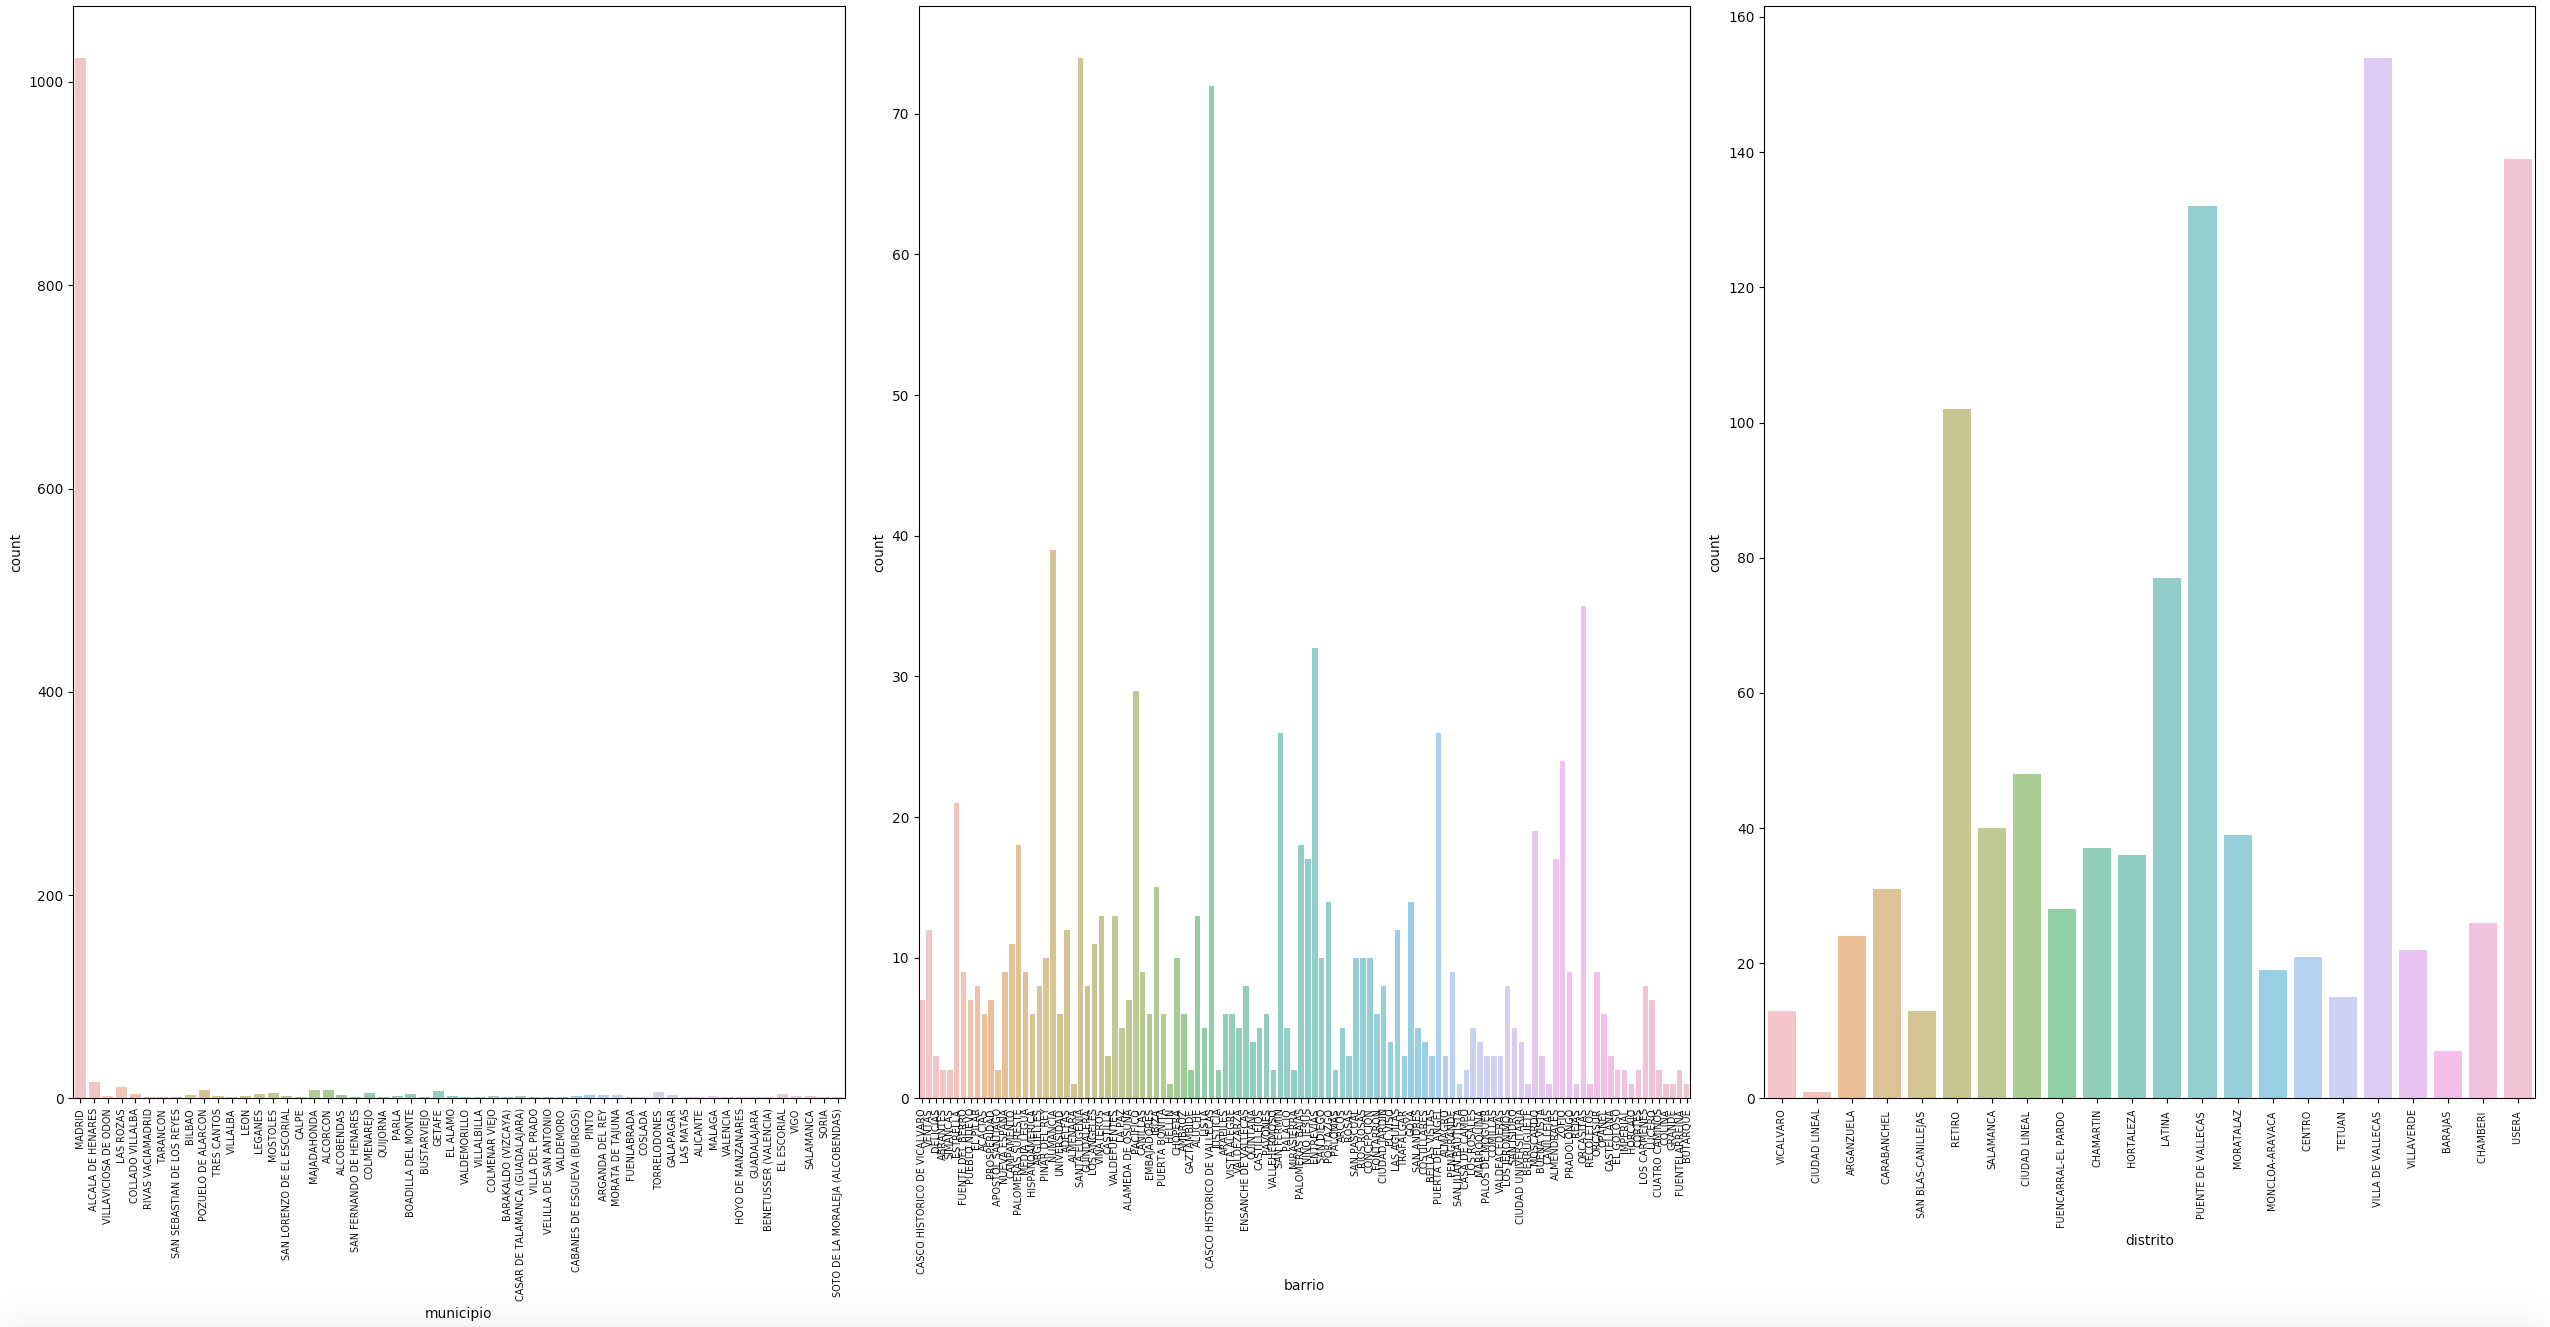
\includegraphics[height=\textheight, width=\textwidth]{figures/resid_detail}
%         \caption{On the left, city of residency of subjects, the large majority lives in Madrid. Middle figure neighborhood and right figure borough of residence in the city of Madrid. 
%         } \label{fig:incomeresidency}
% \end{figure}


\subsection{Sleep}
\label{ssse:sleep}

Animal studies show that the concentration of Amyloid beta decreases drastically during sleep, suggesting that the removal of metabolic debris could take place during sleep \cite{kang2009amyloid}, \cite{xie2013sleep}. Poor sleep is linked to AD, in particular, the sleep–wake cycle has an effect on levels of amyloid-beta in the brain \cite{ju2014sleep}. In a study that measured the association between amyloid-beta burden, relative to baseline, and sleep deprivation in 20 healthy controls \cite{shokri2018beta}, researchers reported that one night of sleep deprivation is sufficient for a significant increase in amyloid-beta in the right hippocampus and thalamus. This is in line with previous mouse studies that showed that brain levels of beta-amyloid decrease during sleep \cite{xie2013sleep}. Tau protein is also affected in altered sleep cycles, a recent study \cite{holth2019sleep} shows that excessive amounts of tau in the cerebral spinal fluid and spinal cord in extremely sleep-deprived adults. The increase in tau surpassed a $30\%$ increase in the Amyloid beta peptide. 

The two most important hallmarks of AD -amyloid plaques and tau aggregates- are thus, affected by sleep. 
However, the causal link sleep-AD is unclear; Does lack of sleep causes AD or is the pathology responsible for disrupting the sleeping cycle? This chicken-and-egg problem can not be solved with correlational neither with meta-analysis studies. Nevertheless, meta analysis \cite{bubu2016sleep} have confirmed the association between sleep deprivation and cognitive impairment or AD, and can furthermore approximate an "average" magnitude of effect. More importantly, sleep-wake cycles can be approached as a modifiable risk factor of interest in the prevention of AD. 
%https://www.sciencenews.org/article/sleep-brain-alzheimers-plaques-protein
 
Figure \ref{fig:sleep} depicts features related to sleep patterns in the \emph{Vallecas} cohort. Daily naps are less common than what it could be expected from a Spaniard population aged 70 or more. $37\%$ of subjects do not take any nap at all, $24\%$ of subjects sleep daily between 15 and 30 minutes and the $17$ report to take naps of at least one hour a day. The majority of subjects report remembering their dreams $67.7\%$ versus $32\%$ that do not. The majority of subjects ($60\%$) report to snore during sleep. 
% YS remove TBI of charts
\begin{figure}[H]
        \centering
        \includegraphics[keepaspectratio, width=\linewidth]{figures/Fig_sleep}
        \caption{Histogram of sleep variables in the \emph{Proyecto Vallecas} dataset in the first year. From left to right and up to the bottom, number of hours of sleep during the day ($\mu=0.45, \sigma=1$), tingling during sleep (0 No, 1 Yes), movements during sleep (0 No, 1 Yes), number of hours of night sleep ($\mu=6.8, \sigma=1.3$), deep sleep (1 Light, 2 Moderate, 3 Deep), remember dreams (0 No, 1 Yes), snoring (0 No, 1 Yes, 2 snore and difficult breathing), noises during sleep (0 No, 1 Yes), sufficient sleep (0 No, 1 Yes).} 
        \label{fig:sleep}
\end{figure}


\subsection{Life style: food and diet, physical exercise and social bonding}
\label{ssse:life}

In a recent study performing PET imaging repeated in three years time, volunteers aged 30-60 with no symptoms of dementia when the study began were divided into two groups: 34 people ate a Mediterranean diet (high fruits, vegetables, lean protein) and 36 people ate a Western diet (high in saturated fats and refined sugar). Researchers reported that at the onset of the study, people that ate Western diet already had more beta-amyloid deposits than those who ate a Mediterranean diet. The follow up scans showed an even greater difference in beta-amyloid deposits in the two groups, controlling for sex, age and genotype factors \cite{berti2018mediterranean}.

AD leads to metabolic impairment which is visible in reductions in cerebral glucose uptake. The early detection of decline in brain glucose metabolism could be of interest as a potential therapeutic intervention of AD. Since hypometabolism precedes clinical symptoms of AD, enhancing glucose uptake \cite{duran2016glucose}, for example with ketone bodies \cite{gasior2006neuroprotective}, could have a neuroprotective effects. The ketogenic diet (high in animal fat and low in carbohydrates) is a clinically established nonpharmacological treatment for epilepsy \cite{vining1998multicenter}. It is plausible that neuroprotective effects (enhanced cell energetics) observed in epilepsy could be of use in the treatment of neurodegenerative diseases, protecting against neuronal death through antioxidant and anti-inflammatory actions. From a biochemical standpoint, replacing glucose by ketone bodies can be seen as a sensible choice and there is research reporting an improvement in cognitive functioning in older adults with memory disorders followed by increases of plasma ketone body via the administration of medium chain triglycerides (MCTs) \cite{reger2004effects}. However, the potential downstream costs associated with the adherence to strict ketogenic nutritional recommendations are not fully understood. 

% Food
Figure \ref{fig:food} depicts the type of food consumption as reported by the subjects in a questionnaire.

\begin{figure}[H]
        \centering
        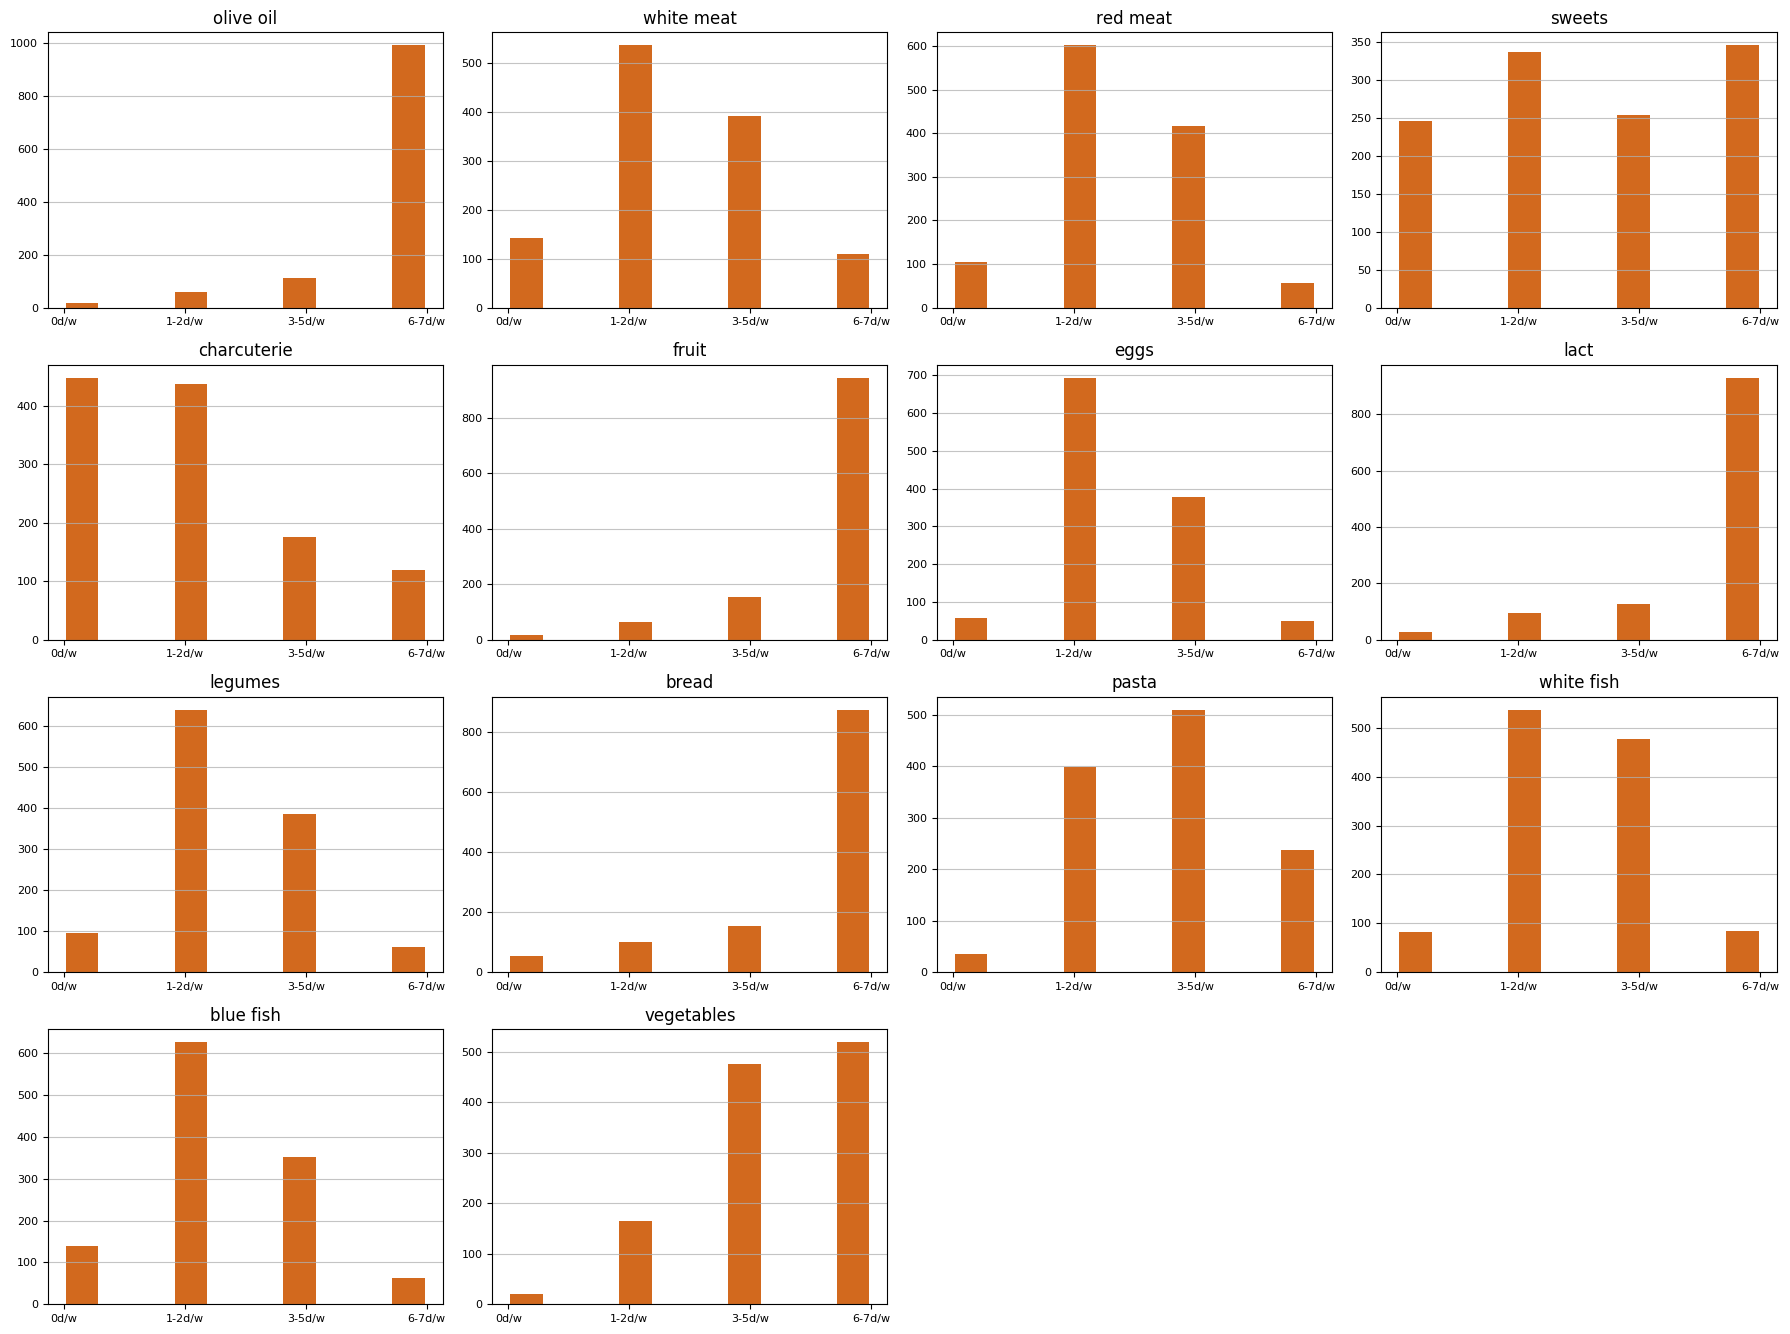
\includegraphics[keepaspectratio, width=\linewidth]{figures/Fig_food}
        \caption{Histogram of type of weekly food consumption reported by the subjects in the first visit. The x-axis of each chart represents how many days a week they consume which type of food. The large majority of subjects report a daily consumption of bread, milk and olive oil. $84\%$ of subjects consume olive oil $6/7$ days a week, $74\%$ bread, $44\%$ vegetables and $29\%$ report consuming sweets $6/7$ days a week.}
        \label{fig:food}
\end{figure}

%Diet
Figure \ref{fig:diet} depicts the type diet based on the reported weekly food consumption. We distinguish between three different diets: diet with a strong glucemic component(carbs, sweets), diet with a strong proteic component or ketogenic (red meat, eggs, fish) and Mediterranean diet (fruit, fish, vegetables). We calculate an score for each diet based on REF-Miguel.

\begin{figure}[H]
        \centering
        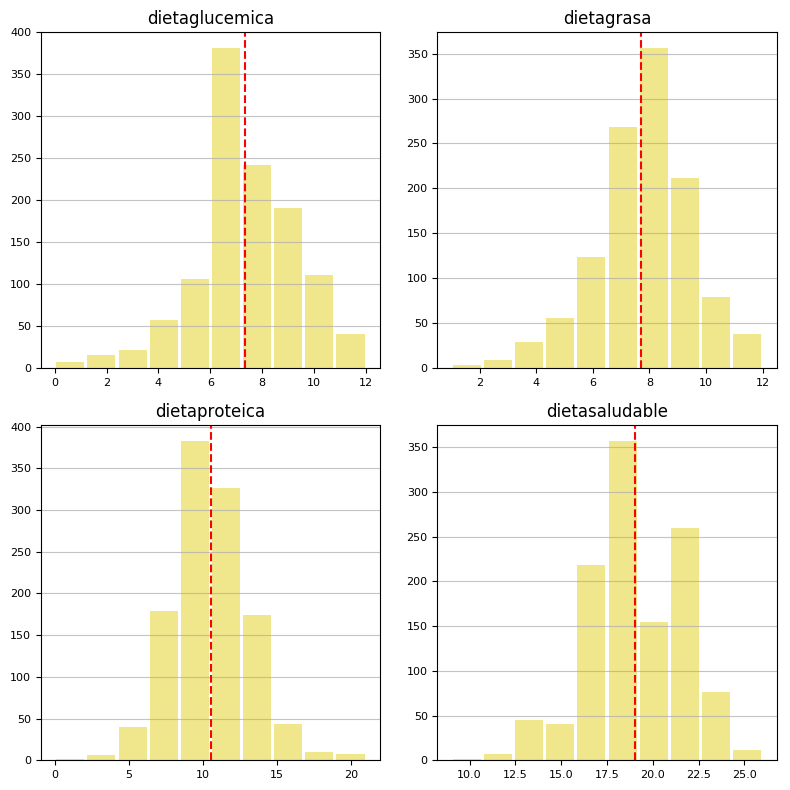
\includegraphics[keepaspectratio, width=.8\linewidth]{figures/Fig_diet}
        \caption{Histogram of type of diet based on weekly food consumption as reported by the subjects in the first visit. The x-axis of each chart represents the score for each type of diet, the larger the score the most prevalent the main component of the diet is in the subject's diet. For example, a subject with a score of 12 in the glucemic diet will likely consume more sweets than a subject a score of 6, by the same token a subject with a large score in the Mediterranean diet will likely consume more fruit and vegetables than a subject with a lower score.} 
        \label{fig:diet}
\end{figure}

%PhysicalExercise_s ['ejfre', 'ejminut']
%YS: fig left, cambio 1,2 por dias a la semana
Studies have shown a beneficial effect of physical exercise in the aging brain, reporting increasing executive functioning and reduction in the expected with age decline of white and gray tissue density with increased fitness \cite{colcombe2003aerobic}. The effects of physical exercise in white matter of the aging brain are particularly interesting. Overall, white matter volume variations seems to be more contained than gray matter volume variation during healthy aging \cite{bartzokis2003white}. However, white matter decline is better observed with DTI-based measures rather than conventional T1-weighted imaging \cite{giorgio2010age}.
%Although there is variation among brain regions, it is thought that  We will explore this hypothesis in the future when we have available the segmentation of all the years.
%YS yes!!

Figure \ref{fig:phys} depicts features related to physical exercise. The subjects were asked the frequency in days per week of their physical exercise and the duration of the sessions.
\begin{figure}[H]
        \centering
        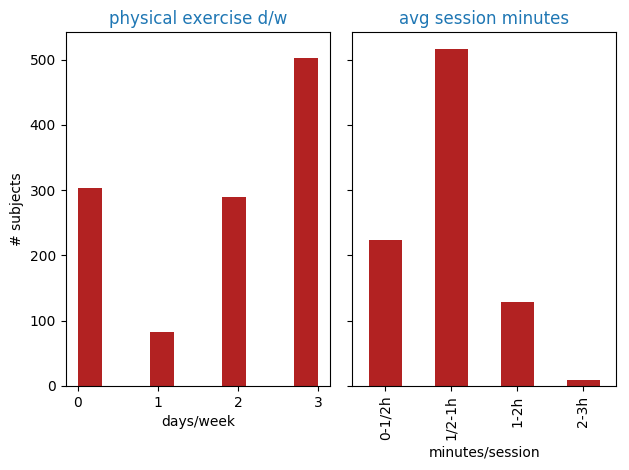
\includegraphics[keepaspectratio, width=0.6\linewidth]{figures/Fig_phys}
        \caption{Histogram of features related to physical exercise. On the left days/week that subjects report to practice physical exercise, and on the right the average duration of the sessions (\emph{less than 30 minutes, less than one hour, between one and two hours and more than two hours})} 
        \label{fig:phys}
\end{figure}

%EngagementExternalWorld_s ['a01', 'a02', 'a03', 'a04', 'a05', 'a06', 'a07', 'a08', 'a09', 'a10', 'a11', 'a12', 'a13', 'a14']
% social bonding

Psychosocial factors such as a rich social network, social engagement and mentally stimulating activities are commonly held as protective factors against dementia/AD. Loneliness, depression, living alone are psychosocial stressors that can increase the risk of developing AD \cite{johansson2013common}, \cite{sindi2015advances}. Figure \ref{fig:engage} depicts features related to engagement with the external world of the subject. In particular, doing creative activities, going out with friends, travel and tourism, community activities (e.g. cultural associations and NGO), going to church, visit social club, go to the movie theater or art shows, go to sport events, how often listens to music, how often watches/listens TV/radio, reading habits (books, newspaper, magazines), and use of the Internet and information technologies.
%EngagementExternalWorld_s ['a03' amigos, 'a04' travel, 'a05' ong, 'a06' church, 'a08' cine, 'a09' sport, 'a10' music, 'a11' tv, 'a12' read, 'a13' internet] 
Of interest, church goers are a minority in our population, $75\%$ never go to church, $17\%$ that go a few times and $8\%$ go often. $86\%$ habitually watches the TV or listens to the radio, $68\%$ read books or magazines often and only $29\%$ use the Internet often.

\begin{figure}[H]
        \centering
        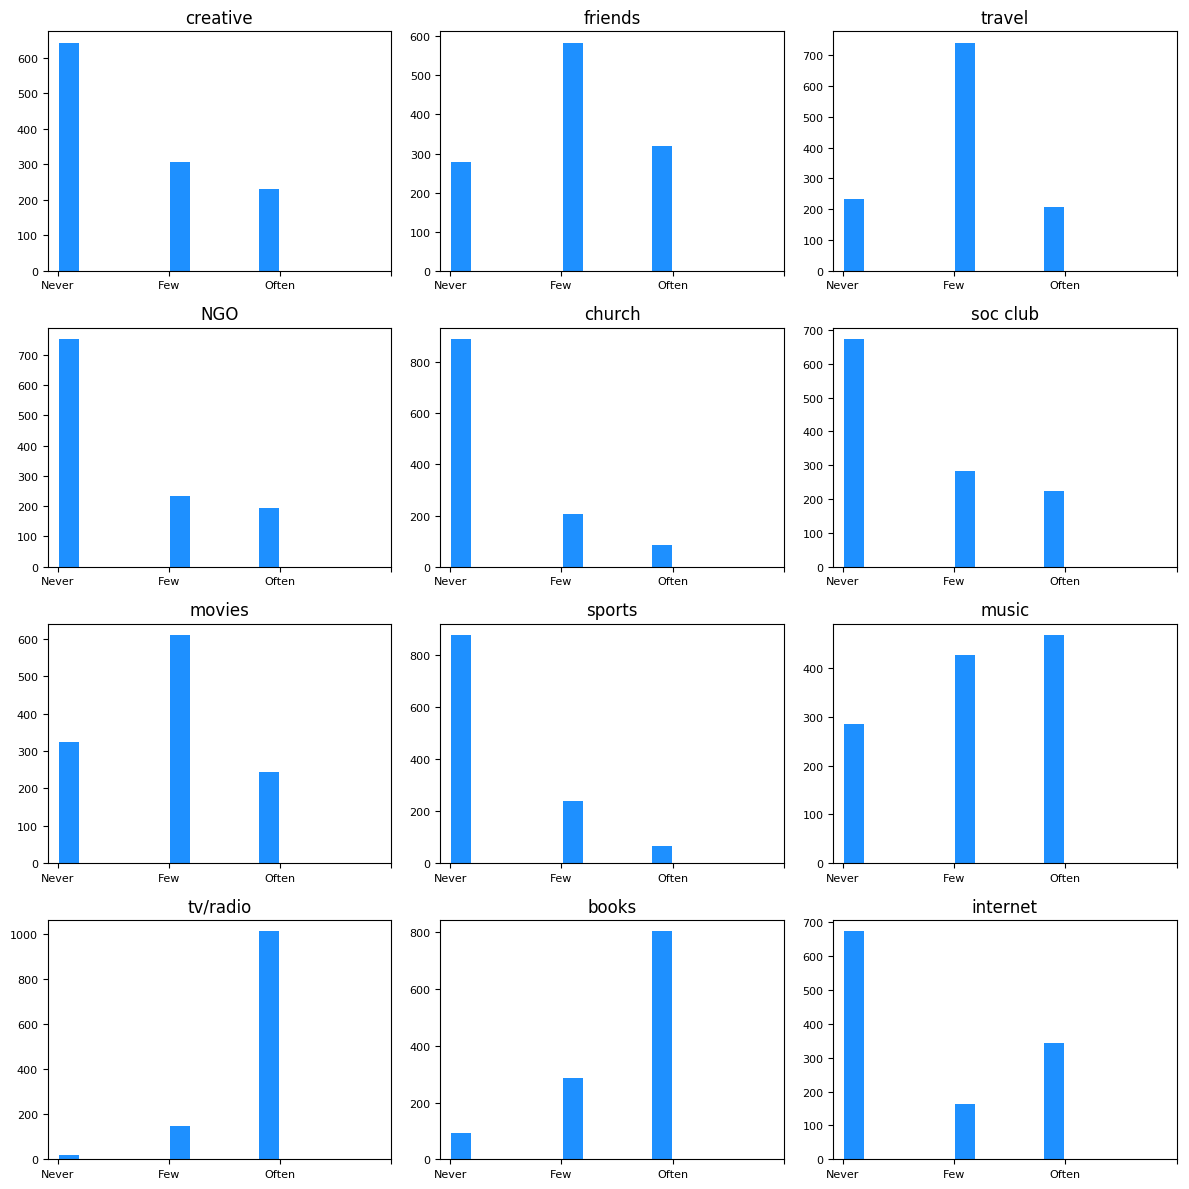
\includegraphics[keepaspectratio, width=\linewidth]{figures/Fig_engage}
        \caption{Histogram of features that reflect engagement with the external world from the part of the subject. From top down and left to right the charts depict the number of subjects that get involve in creative activities, going out with friends, travel and tourism, community activities (e.g. cultural associations and NGO), going to church, visit social club, go to the movie theater or art shows, go to sport events, how often listens to music, how often watches/listens TVradio , how often reads (books, newspaper, magazines), how often uses the internet.} 
        \label{fig:engage}
\end{figure}


\subsection{Cardiovascular and cerebrovascular pathologies}
\label{ssse:cardio}
% Cardiovascular_s ['hta', 'hta_ini', 'glu', 'lipid', 'tabac', 'tabac_cant', 'tabac_fin', 'tabac_ini', 'sp', 'cor', 'cor_ini', 'arri', 'arri_ini', 'card', 'card_ini', 'tir', 'ictus', 'ictus_num', 'ictus_ini', 'ictus_secu']

A recent genome-wide study has been able to identify genetic variants that confer a risk of both cardiovascular disease and Alzheimer's disease \cite{broce2019dissecting}. Vascular risk factors for AD such as diabetes, heart failure, stroke, hypertension and smoking among others could be involved in cerebrovascular dysfunction and AD pathology. Cardiovascular risk factors and their associated brain mechanisms are believed to play a role in the onset of AD. 
A better understanding of the interplay between cardiovascular disorders is not only beneficial from a clinical perspective but also from a prevention point of view, suggesting behavioral interventions (smoking cessation, healthy diet etc. ) in early adult life \cite{de2010cardiac}.  

Thyroid hormones have a significant impact on the cardiac system (excess thyroid hormone affects cardiovascular function \cite{klein2007thyroid}).
%, subjects also reported whether they suffer from hyper(hipo)thyroidism 
Stroke is a risk factor for coronary heart disease and subjects were asked if they had in the past hemorrhagic or ischemic cerebral ictus. Ischemic stroke and AD share pathophysiological mechanisms such as inflammation, immune exhaustion and neurovascular damage \cite{lucke2015common}. 
The causality narrative between AD and hemorrhagic stroke seems to be reversed (AD causes X, rather than the usual search of factor X that causes AD), patients who had Alzheimer's disease are at the highest risk of hemorrhagic stroke \cite{wang2014newly}.

Figure \ref{fig:cardio} depicts features related to the cardiovascular health self reported in the \emph{Vallecas} cohort. The subjects were asked whether they suffer hypertension, angina and heart attack, glucose metabolism disorders, dyslipidemia (an abnormal amount of lipids in the blood), arrhythmias and smoking habits. The majority of subjects report to have hypertension $53\%$ vs $47\%$, this is in line with larger studies, for example in \cite{grau2011cardiovascular} 28,887 participants in Spain aged 35-74, high blood pressure was present in $47\%$ of men and $39\%$ of women, in \cite{lacruz2015prevalence}.
$27\%$ of the participants declared to be smokers and $33\%$ ex-smokers.


 %total cholesterol ≥ 250 mg/dL (43% and 40%, respectively), 
 %obesity (29% and 29%, respectively), tobacco use (33% and 21%, respectively), and diabetes (16% and 11%, respectively). Total cholesterol ≥ 190 and ≥ 250 mg/dL were the respective minimum and maximum coefficients of variation (7%-24% in men, 7%-26% in women). Average concordance in lipid measurements between laboratories was excellent. 
%of note the self reported hypertension is inferior to population studies in which the blood pressure is actually measured mean systolic $\geq140$ mmHg and/or diastolic BP (DBP) $\geq90$ mmHg and/or use of antihypertensive medication \cite{lacruz2015prevalence}. 

%https://www.brightfocus.org/alzheimers/article/weight-risk-factor-alzheimers-disease

%https://www.isglobal.org/en/new/-/asset_publisher/JZ9fGljXnWpI/content/cardiopatia-isquemica-demencias-e-ictus-se-situan-como-las-principales-causas-de-muerte-en-espana

%YS: change arrythmia in pic for stroke 3 top
\begin{figure}[H]
        \centering
        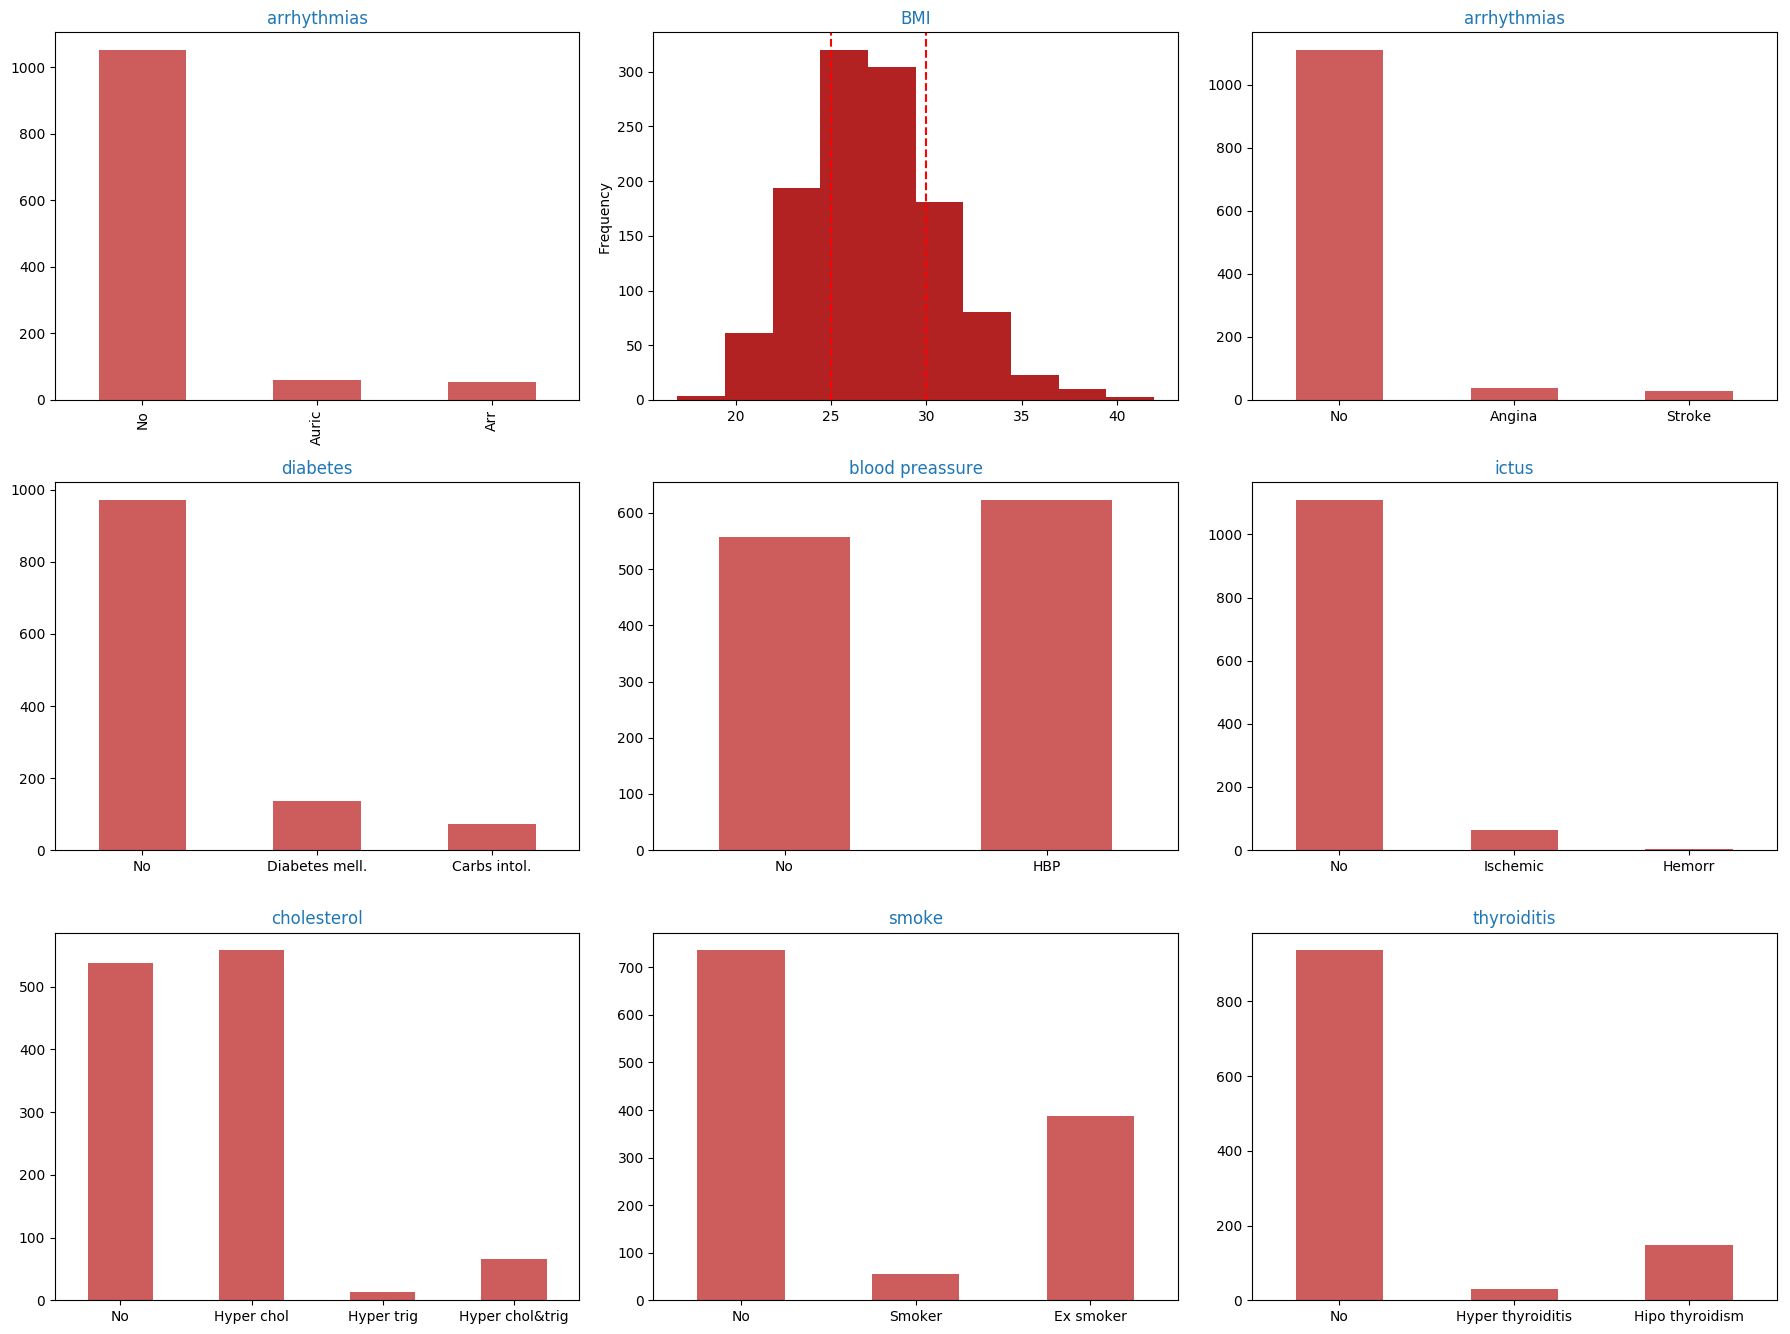
\includegraphics[keepaspectratio, width=\linewidth]{figures/Fig_cardio}
        \caption{Histogram of features related to cardiovascular health. From top down and left to right: arrythmias (\emph{No Arrhythmia, Atrial fibrillation, Arrhythmia}), body mass index, heart stroke (\emph{No past strokes, Angina, Stroke}), diabetes (\emph{No diabetic, diabetes mellitus, intollerance to carbs}), hypertension, ictus history (\emph{No, Ischemic, Hemorrhagic}), cholesterol (\emph{No cholesterol, hyper cholesterol, Hyper triglycerides, both hyper cholesterol and triglycerides}), Smoke (\emph{Non smoker, Smoker, Ex-smoker}), thyroiditis (\emph{No thyroiditis, Hyper thyroiditis, hipo thyroiditis}). } 
        \label{fig:cardio}
\end{figure}

% Pass on sp (you think you are overweighted?) and use If your BMI is 25.0 to <30, it falls within the overweight range. If your BMI is 30.0 or higher, it falls within the obese range

%\subsection{Traumatic brain injury}
%\label{ssse:tbe}
%TraumaticBrainInjury_s ['tce', 'tce_con', 'tce_ini', 'tce_num', 'tce_secu']

Traumatic brain injury (TBI) is associated with long-term and acute disorders whose onset and ethiology are insufficiently understood. Violent head displacements in vulnerable brains is a precursor of dementia. A plausible mechanism of transmission is the propagation of abnormal proteins along damaged white matter pathways. Furthermore, TBI can initiate cerebrovascular pathology, which in turn could mediate in neurodegeneration including AD-like dementias \cite{ramos2018traumatic}. See \cite{mendez2017relationship} for a summary of recent research on the TBI-dementia link. 

Figure \ref{fig:tce} shows the distribution of episodes (at least one) of traumatic brain injury in the \emph{Vallecas} cohort. 

\begin{figure}[H]
        \centering
        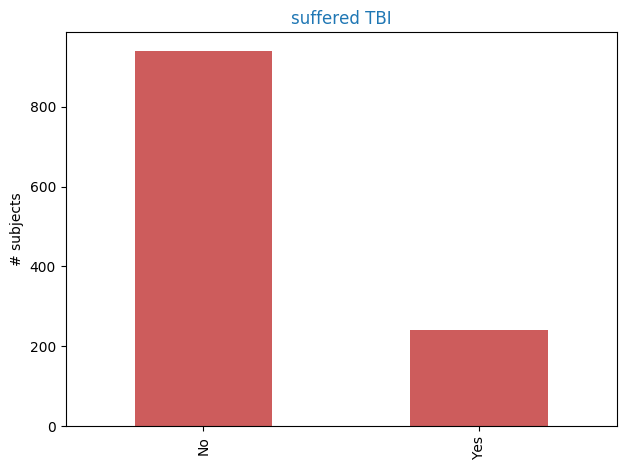
\includegraphics[keepaspectratio, width=0.4\linewidth]{figures/Fig_tce}
        \caption{Histogram of traumatic brain injury. $20\%$ of subjects declared to have suffered in the past an episode of traumatic brain injury of unspecified seriousness.} 
        \label{fig:tce}
\end{figure}

%%%%%%%%%%%%%%%%%%%%%%%%%%%%%%%%%%%%%%%%%%%%%%%%%%%%%%%%%
%%%%%%%%%%%%%%%%%%%%%%%%%%%%%%%%%%%%%%%%%%%%%%%%%%%%%%%%%
\section{Exploratory Data Analysis longitudinal variables}
\label{se:eda_long}
%'CognitivePerformance', 'Diagnoses', 'Neuropsychiatric', 'QualityOfLife', 'Genetics_s', 'SCD', 'Demographics', 'Cardiovascular_s', 'PhysicalExercise_s', 'Sleep_s', 'Anthropometric_s', 'Diet_s', 'SocialEngagement_s', 'TraumaticBrainInjury_s', 'Demographics_s', 'EngagementExternalWorld_s'
In this section we study the evolution of the variables measured in the \emph{Vallecas} study. We dedicate the first section \ref{sse:miss} to comment on the method employed to deal with data missing to next discuss the evolution of the variable. 
We will study the progression of the longitudinal variables for those subjects that did not miss any visit of their 6 visits (complete-case-analysis). Thus, from an initial number of 1180 subjects that came to their first visit, we will study the time series for the subset of subjects that came to all their visits from year 1 to year 6, which makes a total of 457 subjects span over a 6 year period.
The adjustment methods for missing data used here is complete-case analysis, that is, participants with missing data are simply excluded from the analysis. It ought to be noted that this is a methodological choice and other strategies are also possible, see \cite{national2010prevention} for a recent report with recommendations for missing data in clinical trials published by the National Research Council (NRC). 

The longitudinal variables are studied as time series of length 6 (number of yearly visits) with 457 observations for each time point.  MRI data is shown in section \ref{sse:mri}, neuropsychiatric features in section \ref{sse:neupsy}, quality of life in section \ref{sse:qol}, cognitive performance tests are shown in section \ref{sse:cogper} and the evolution of the diagnosis in section \ref{sse:diagn}.

\subsection{Treatment of missing imputation}
\label{sse:miss}
%check if subjects go away have a profile
Just like in any other longitudinal study, drop out is an important concern. The causes for missing visits can be related to first and foremost the voluntary and non remunerated design of the project and the age of the subjects (70 at the inception). The discontinued participation can also be caused by the diagnosis of dementia, possibly in the study clinical assessment.

Missing data compromises statistical inference and represents a serious limitation for drawing conclusions \cite{little2012prevention}. 
Although there are different methods for completion of missing data e.g. Maximum likelihood, Bayesian and multiple imputation \cite{hogan2004handling}, the effectiveness of a statistical method relies upon the plausibility of its assumptions. Thus, it is desirable to have evidence of the mechanisms leading to missing data. There are two major possible scenarios: data missing are completely random and data missing are not at random. The first case is less stringent because it could be possible to infer that the outcomes of participants that dropped out are not significantly different from those that did not drop out. In the second case, data are missing not at random, outcomes are likely to be different from those of similar participants who did not drop out. In the latter case, statistical model need to make additional assumptions. 

There are several statistical methods to handle drop out effects \cite{hogan2004handling}, however since the attrition rate is severe (1180 to 491 in year 6) we opt first to investigate whether the sample changes according to specific patterns, in which case we would not attempt to complete the missing data and we would rather select the subset of subjects that did not miss any visit (471 subjects did not miss any visit from year 1 to year 6).

%avatars 
%https://www.123rf.com/photo_54326404_stock-vector-set-of-characters-in-a-flat-style-older-people-in-different-costumes-grandparents-in-cartoon-flat-st.html?fromid=eDZxWk1FN08rcnBqencvNDlIVlZ2dz09
Figure \ref{fig:abuelos} depicts the drop-out handling the \emph{Vallecas} longitudinal study longitudinal study. For example, to test  the drop out in year 2 we compare the means between the two groups: $(1)$ and $(2,3,4,5,6,7)$ because subject 1 drop the study in year 2, to test the drop out in year 4 referred to year 1 we compare between the groups: $(1,3)$ and $(2,4,5,6,7)$. 
\begin{figure}[H]
        \centering
        \includegraphics[keepaspectratio,width=0.95\linewidth]{figures/abuelos}
        \caption{Sketch of the drop out handling in the \emph{Vallecas} longitudinal study. Only the subjects that did not miss any of their six visits are considered for the longitudinal analysis described in this section.} 
        \label{fig:tce}
\end{figure}

Table \ref{tab:testloyals} shows the statistical test to study whether the subjects that drop out are significantly different than those that remain in the study. While for home residency or APOE there is no evidence of difference between the "remainers" and the "leavers", for a number of other features such as age, educational level or familal AD we find significant differences between the two  groups. Note that we perform a two samples t-test comparing the subjects were present at year 1 and year k $(k=2..6)$ versus subjects present at year 1 but missed year k. The actual size of the groups is indicated in the second row, for example 689 missed their 6th visit and 491 came to their 6th visit. 

\begin{table}
  \centering
\begin{tabular}{cccccc} \toprule
    {Feature}   & {${Y1-Y2}$} & {${Y1-Y3}$} & {${Y1-Y4}$} & {${Y1-Y5}$} & {${Y1-Y6}$} \\ 
                & N={${964,216}$} & N={${865,315}$} & N={${773,407}$} & N={${704,476}$} & N={${491,689}$} \\  \midrule
    {feature1}  & & & & &  \\
    {${Y2}$}    & & & & &  \\ %\midrule
    {${Y3}$}    & & & & &  \\  
    {${Y4}$}    & & & & &  \\ 
    {${Y5}$}    & & & & &  \\
    {featureN}  & & & & &  \\ \bottomrule
\end{tabular}
\caption{T-test for the means of two independent samples scores in year 1 for subjects that participated in year $k, (k=2,...,6)$, versus those that missed their \emph{k-th} visit.}\label{tab:testloyals}
\end{table} 
The complete-case analysis followed here to handle missing longitudinal data is justified on the basis of the non randomness of the missing data. As table \ref{tab:testloyals} tries to convey, outcomes (e.g. age, educational level, familal AD) are likely to be different from those of similar participants who did not drop out. 

Note that we opt for complete-case analysis for longitudinal data, that is, an entire missing visits, but 
we used the much less stringent Multiple Imputation (MI) \cite{buuren2010mice} approach for dealing with missing data within a subject's visit.
%Models that are based on the assumption that the data are not missing at random must make further assumptions about the effect of such possibilities.
%The assumption that analysis methods can com- pensate for such missing data are not justified

\subsection{MRI}
\label{sse:mri}
Here we show the automated segmentation of all subjects with MRI in the first year, so far we present the results for brain extraction for the first year. We plan to show segmentation of subcortical structure for all the years in the short future. Of note, the imaging data has not been stored, let alone preprocessed, with the minimum quality requirements for a project of of such volume and complexity. This is delaying and the work that we intend to show here.

The segmentation goes through the following stages:
\begin{enumerate}  
  %0 The input image is copied in .anat and renamed {T1}.nii.gz (-t T1,T2,PD), we work with T1 now
  \item \textbf{Reorientation} to the standard (MNI) orientation
  %, \emph{fslreorient2std} it swaps axes around maintaining the correct left-right relationships so that x=left-right, y=anterior-posterior and z=superior-inferior. 
  %size T1 < T1_orig== T1_fullfov, T1 reoriented and cropped is small in size than the original image because we cut the neck. e. T1.nii.gz is the averaged and aligned image file. 
  \item \textbf{Cropping} to remove the neck, this is a necessary step prior to brain extraction. 
  %\emph{robustfov} looks at axial slices in the superior direction (starting at the edge of the volume and moving towards the centre) and determines whether a slice contains only noise or signal plus noise. Once it finds the first consecutive slices that contain signal plus noise it then takes that as the position of the top of the head and then extracts a fixed size of FOV in the superior-inferior direction down from the top of the head, which should cover the brain but stop short of the jaw and neck
  \item \textbf{Bias field correction} 
  %  I used strongbias = no good if the field is not strong which is good for 1-5T. 
    %For high-field or multi-coil array is better to use strongfield=yes. 
    %For my MRI, 3T and not multi-coil what to use?
  %The bias-corrected version of the image is called T1_biascorr
  \item \textbf{Registration} to standard space computing both linear registration (FLIRT algorithm) and non-linear registration (FNIRT algorithm)
  %do_nonlinreg=yes call to [fnirt], [flirt] is always run also for non linear registration
  %creates the images: T1_to_MNI_lin (the result of the linear reg), T1_to_MNI_nonlin(the result of the non linear reg)
  %T1_to_MNI_nonlin_field (non-linear warp field) , T1_to_MNI_nonlin_jac (Jacobian of the non-linear warp field)
  %and T1_vols.txt containing a scaling factor and brain volumes, based on skull-constrained registration, suitable for head-size normalisation (as the scaling is based on the skull size, not the brain size). 
  \item \textbf{Brain Extraction} in two steps. First, the BET algorithm obtains a brain mask which can be coarse to then perform the brain extraction transforming standard-space mask to the input image using the FNIRT (non-linear) registration.
  %This step can be interactive changing the threshold : You must adjust the threshold for the extraction (-f) to assure that the skull is removed while the cortical surface is left in tact. This will require running BET multiple times to assure that it is satisfactory. 
  %run $FSLDIR/bin/bet ${T1} ${T1}_initfast2_brain -m -f 0.1 (by default betfparam=0.1)
  % 0.1 is overincusive, it will get a very rough brain which means it will likely get portions of the skull(the larger the f eg 0.8 the most brain restricted) but we use 0.1 because we refibne after with FNRIT
  %produces: T1_biascorr_brain and T1_biascorr_brain_mask
  \item \textbf{Tissue Segmentation} (FAST algorithm)
  %produces: T1_biascorr - refined again in this stage, (CSF) T1_fast_pve_0, (Gray) T1_fast_pve_1, (White)T1_fast_pve_2 - partial volume segmentations (CSF, GM, WM respectively) and T1_fast_pveseg - a summary image showing the tissue with the greatest partial volume fraction per voxel
  \item \textbf{Subcortical Segmentation} (FIRST algorithm)
  %T1_subcort_seg - summary image of all subcortical segmentations, T1_biascorr_to_std_sub.mat - a transformation matrix of the subcortical optimised MNI registration
  %All the other ouputs in first_results subdir: T1_first_all_fast_firstseg == T1_subcort_seg and btk, vbars for each region, need to be converted to .nii
\end{enumerate}

We show the results for brain extraction, tissue segmentation (CSF, white and gray matter) and subcortical segmentation (thalamus, putamen, hippocampus, accumbens, pallidum, caudate, amygdala) for a total of 979 MRIs in the first year. 

\paragraph*{Brain extraction}

Research shows that the growth rate of the brain slowly declines declines from the first year of birth (it increases dramatically during), brain volume reaches its maximum at the age of 40 years to then decline by $5\%$ per decade, the decline is thought to accelerate at around 70 years \cite{peters2006ageing}.

Figure \ref{fig:boxbet} shows the results of the brain extraction algorithm. First, the BET algorithm obtains a brain mask to then perform the brain extraction transforming standard-space mask to the input image using a non-linear registration algorithm.

The brain's size is expressed in mm${^3}$ in native space (left) and scaled in MNI space (right). The average brain size is around 1,000 cm${^3}$ or 1000,000 mm${^3}$ which reflects the age and the gender unbalance of the sample.

\begin{figure}[H]
        \centering
        \includegraphics[keepaspectratio, width=0.6\linewidth]{figures/boxplot_Nonebrain}
        \caption{The figure shows the box plot of the size of the brain in mm${^3}$ both in native space (left) and in the normalized MNI space (right).} 
        \label{fig:boxbet}
\end{figure}

\paragraph*{Segmentation of brain tissue}
%fsleyes T1_fast_restore.nii.gz T1_fast_pve_0.nii.gz -cm green -dr 0.5 1 T1_fast_pve_1.nii.gz -cm blue-lightblue -dr 0.5 1 T1_fast_pve_2.nii.gz -cm red-yellow -dr 0.5 1
Figure \ref{fig:tissueseg} shows the segmentation based on tissue (CSF (green), Gray matter(blue); White matter (red-yellow)) of one subject of the \emph{Vallecas Project}.

\begin{figure}[H]
        \centering
        \includegraphics[keepaspectratio, width=\linewidth]{figures/tissueseg}
        \caption{Example of tissue based segmentation of one subject in her first visit. } 
        \label{fig:tissueseg}
\end{figure}
%fsleyes ../T1_fast_restore.nii.gz T1_first_all_fast_firstseg.nii.gz -cm Red-Yellow -dr 0 118

Figure \ref{fig:boxtissue} shows the boxplot of the segmentation of tissues of the 957 MRIs in the first year \emph{Vallecas Project}. CSF volume on the left, gray matter center and white matter on the right. All volumes are expressed in mm${^3}$.


\begin{figure}[H]
        \centering
        \includegraphics[keepaspectratio, width=\linewidth]{figures/boxplot_no_outlierstissue}
        \caption{Boxplot of volume in mm${^3}$ for the tissue based segmentation (CSF, Gray matter, White matter) for all the MRIs performed during the first year of \emph{Vallecas Project}. Outliers containing extreme values were removed using an automated issue identification algorithm.} 
        \label{fig:boxtissue}
\end{figure}

Figure \ref{fig:kde_3_tissues} shows the histogram and the Kernel Density Estimate (a non-parametric way to estimate the probability density function of a random variable) of the segmentation of tissues of the 957 MRIs in the first year \emph{Vallecas Project}. The volume is expressed in mm${^3}$.
\begin{figure}[H]
        \centering
        \includegraphics[keepaspectratio, width=\linewidth]{figures/kde_3_tissues}
        \caption{Histogram and KDE in cm${^3}$ for tissue based segmentation (CSF, Gray matter, White matter) for all the MRIs performed during the first year of \emph{Vallecas Project}. Outliers containing extreme values were removed using an automated issue identification algorithm.} 
        \label{fig:kde_3_tissues}
\end{figure}


\paragraph*{Segmentation of brain subcortical structures}

Figure \ref{fig:subcorseg} shows the segmentation based of the subcortical structures: Thalamus, Putamen, Hippocampus, Accumbens, Pallidum, Caudate, Amygdala and Brain stem of one subject of the \emph{Vallecas Project}. The statistical analysis of all the subjects in the first year visit  will be ready very SOON! 

\begin{figure}[H]
        \centering
        \includegraphics[keepaspectratio, width=\linewidth]{figures/subcorseg}
        \caption{Segmentation of subcortical structures Thalamus, Putamen, Hippocampus, Accumbens, Pallidum, Caudate, Amygdala of one subject of the \emph{Vallecas Project}. } 
        \label{fig:subcorseg}
\end{figure}

Figure \ref{fig:boxsubcor} shows the boxplot of the segmentation of subcortical structures of the 957 MRIs in the first year \emph{Vallecas Project}. The volume is expressed in mm${^3}$.
\begin{figure}[H]
        \centering
        \includegraphics[keepaspectratio, width=\linewidth]{figures/boxplot_no_outlierssubcortical}
        \caption{Boxplot of volume in mm${^3}$ of the bilateral subcortical segmentation for all the MRIs performed during the first year of \emph{Vallecas Project}. Outliers containing extreme values were removed using an automated issue identification algorithm. The subcortical structures represented are Thalamus, Putamen, Hippocampus, Accumbens, Pallidum, Caudate, Amygdala.} 
        \label{fig:boxsubcor}
\end{figure}

Figure \ref{fig:kde_subcortical} shows the histogram and the Kernel Density Estimate (a non-parametric way to estimate the probability density function of a random variable) of the segmentation of subcortical structures of the 957 MRIs in the first year \emph{Vallecas Project}. The volume is expressed in mm${^3}$.
\begin{figure}[H]
        \centering
        \includegraphics[keepaspectratio, width=\linewidth]{figures/kde_subcortical}
        \caption{Boxplot of volume in mm${^3}$ of the bilateral subcortical segmentation for all the MRIs performed during the first year of \emph{Vallecas Project}. Outliers containing extreme values were removed using an automated issue identification algorithm. The subcortical structures represented are Thalamus, Putamen, Hippocampus, Accumbens, Pallidum, Caudate, Amygdala.} 
        \label{fig:kde_subcortical}
\end{figure}

%%%%%%%%%%%%%%%%%%%%%%%%%%%%%%%%%%%
\subsection{Cognitive Performance}
\label{sse:cogper}
Figure \ref{fig:cogperyears} plots the evolution of four cognitive performance tests. Clockwise and starting on  the top left chart: number of words that start by the letter "p" in one minute, number of animals recalled in one minute, score of speed processing of symbols and the score in the mini-mental examination (MMSE).

% _loyals only subset of six visits figaname for entire dataset longitudinal
\begin{figure}[H]
    \centering
    \begin{subfigure}[t]{0.4\textwidth}
        \centering
        \includegraphics[height=2.1in]{figures/p_visita_loyals}
        \caption{Histograms of the score of the number of words starting by a letter for each year's test.}
    \end{subfigure}
    \hfill
    \begin{subfigure}[t]{0.4\textwidth}
        \centering
        \includegraphics[height=2.1in]{figures/animales_visita_loyals}
        \caption{Histograms of number of animals recalled each year's test.}
    \end{subfigure}%\quad
    
     \begin{subfigure}[t]{0.4\textwidth}
        \centering
        \includegraphics[height=2.1in]{figures/cn_visita_loyals}
        \caption{Histograms of score of speed processing of symbols for each year's test.}
    \end{subfigure}
    \hfill
    \begin{subfigure}[t]{0.4\textwidth}
        \centering
        \includegraphics[height=2.1in]{figures/mmse_visita_loyals}
        \caption{Histograms of score of the MMSE test score for each year's test.}
    \end{subfigure}%\quad
    \caption{Histograms showing the evolution of features related to the cognitive performance of the subjects across the six years of \emph{Vallecas Project} (no missing visits). The scores from left to right and top to bottom refer to: number of words that start by letter p, number of animals, speed processing of symbols and MMSE.}
    \label{fig:cogperyears}
\end{figure}

Figure \ref{fig:cogper4} plots the time series for four measures related to cognitive performance. Clockwise starting top left chart: score of speed processing of symbols, score for the number of animals that the subject can recall in one minute, score for the number of words that start by the letter p in one minute and the score in the mini-mental examination (MMSE).

\begin{figure}[H]
    \centering
    \begin{subfigure}[t]{0.45\textwidth}
        \centering
        \includegraphics[height=2.5in]{figures/p_visita1_years_loyals}
        \caption{Time series (indexed in years) of the  number of words that start by the letter p that subjects can recall in one minute. The statistics for years 1 to 5 (years 6 and 7 are still ongoing): $\mu_{1}=14.01, \sigma_{1}=4.39$, $\mu_{2}=14.16, \sigma_{2}=4.91$, $\mu_{3}=14.91, \sigma_{3}=4.95$, $\mu_{4}=14.71, \sigma_{4}=4.85$,$\mu_{5}=17.07,\sigma_{5}=4.91$, $\mu_{6}=15.43,\sigma_{5}=5.04$.}
    \end{subfigure}
    \hfill
    \begin{subfigure}[t]{0.45\textwidth}
        \centering
        \includegraphics[height=2.5in]{figures/animales_visita1_years_loyals}
        \caption{Time series the  number of animals that subjects can recall in one minute. The statistics for years 1 to 6: $\mu_{1}=14.01, \sigma_{1}=4.4$, $\mu_{2}=14.96, \sigma_{2}=4.90$, $\mu_{3}=18.48, \sigma_{3}=5.40$, $\mu_{4}=18.29, \sigma_{4}=5.54$,$\mu_{5}=18.32,\sigma_{5}=5.50$.}
    \end{subfigure}%\quad
    
     \begin{subfigure}[t]{0.45\textwidth}
        \centering
        \includegraphics[height=2.5in]{figures/cn_visita1_years_loyals}
        \caption{Time series of feature \emph{cn} which measures the speed processing of symbols in a task (attention and velocity). This measure tends to be more stable than other eg Buschke. The statistics for years 1 to 5 (years 6 and 7 are still ongoing): $\mu_{1}=18.71, \sigma_{1}=7.60$, $\mu_{2}=18.70, \sigma_{2}=7.47$, $\mu_{3}=18.81, \sigma_{3}=7.55$, $\mu_{4}=18.54, \sigma_{4}=7.67$,$\mu_{5}=18.05,\sigma_{5}=7.35$.}
    \end{subfigure}
    \hfill
    \begin{subfigure}[t]{0.45\textwidth}
        \centering
        \includegraphics[height=2.5in]{figures/mmse_visita1_years_loyals}
        \caption{Time series of the score of the minimental examination test MMSE. The statistics for years 1 to 5 (years 6 and 7 are still ongoing): $\mu_{1}=28.71, \sigma_{1}=1.40$, $\mu_{2}=28.76, \sigma_{2}=1.51$, $\mu_{3}=28.23, \sigma_{3}=2.00$, $\mu_{4}=28.11, \sigma_{4}=2.28$,$\mu_{5}=27.94,\sigma_{5}=2.45$, $\mu_{6}=28.29,\sigma_{5}=2.03$.}
    \end{subfigure}%\quad
   
    \caption{Time series of cognitive performance across the seven years of \emph{Vallecas Project} of features related to cognitive performance. The x-axis are years from year 1 to year 6 and the y-axis the score. Each plot represents the mean (bold line) and the dispersion or standard deviation (shaded region) across the seven years of \emph{Vallecas Project}.}
    \label{fig:cogper4}
\end{figure}

%YS: Falta hacere esto
Figure \ref{fig:cogperyearsbus}, clockwise and starting in the top left chart: Buschke delayed recalled score, mean, sum and the Buschke Integral score which is explained in a forthcoming paper. We address the reader to the Appendix section for more details).

\begin{figure}[H]
    \centering
    \begin{subfigure}[t]{0.4\textwidth}
        \centering
        \includegraphics[height=2.1in]{figures/fcsrtlibdem_visita}
        \caption{Histograms of the Buschke delayed recall score for each year.}
    \end{subfigure}
    \hfill
    \begin{subfigure}[t]{0.4\textwidth}
        \centering
        \includegraphics[height=2.1in]{figures/bus_meana_visita}
        \caption{Histograms of of the Buschke arithmetic mean for each year.}
    \end{subfigure}%\quad
    
     \begin{subfigure}[t]{0.4\textwidth}
        \centering
        \includegraphics[height=2.1in]{figures/bus_sum_visita}
        \caption{Histograms of of the Buschke sum for each year.}
    \end{subfigure}
    \hfill
    \begin{subfigure}[t]{0.4\textwidth}
        \centering
        \includegraphics[height=2.1in]{figures/bus_int_visita}
        \caption{Histograms of of the \emph{Buschke Integral} score for each year..}
    \end{subfigure}%\quad
   
    \caption{Histograms showing the evolution of features related to the cognitive performance of the subjects across the seven years of \emph{Vallecas Project}. From left to right and top to bottom: 
    Buschke delayed recall score, Buschke arithmetic mean, Buschke sum and \emph{Buschke Integral}.}
    \label{fig:cogperyearsbus}
\end{figure}

Figure \ref{fig:busper4} plots the time series for four measures related to cognitive performance measured using the Buschke test. Clockwise starting top left chart: delayed recalled score, mean, sum and the Buschke Integral score which is explained in a forthcoming paper. We address the reader to the Appendix section for more details).

\begin{figure}[H]
    \centering
    \begin{subfigure}[t]{0.45\textwidth}
        \centering
        \includegraphics[height=2.5in]{figures/fcsrtlibdem_visita1_years}
        \caption{Time series (indexed in years) of Buscke recall delayed score. The statistics for years 1 to 5 (years 6 and 7 are still ongoing): $\mu_{1}=9.02, \sigma_{1}=3.01$, $\mu_{2}=9.44, \sigma_{2}=3.02$, $\mu_{3}=10.10, \sigma_{3}=3.23$, $\mu_{4}=10.44, \sigma_{4}=3.52$,$\mu_{5}=14.76,\sigma_{5}=3.62$.}
    \end{subfigure}
    \hfill
    \begin{subfigure}[t]{0.45\textwidth}
        \centering
        \includegraphics[height=2.5in]{figures/bus_meana_visita1_years}
        \caption{Time series (indexed in years) of the mean of the Buschke score. The statistics for years 1 to 5 (years 6 and 7 are still ongoing): }
    \end{subfigure}%\quad
    
     \begin{subfigure}[t]{0.45\textwidth}
        \centering
        \includegraphics[height=2.5in]{figures/bus_sum_visita1_years}
        \caption{Time series (indexed in years) of the sum of the Buschke score. The statistics for years 1 to 5 (years 6 and 7 are still ongoing):}
    \end{subfigure}
    \hfill 
    \begin{subfigure}[t]{0.45\textwidth}
        \centering
        \includegraphics[height=2.5in]{figures/bus_int_visita1_years}
        \caption{Time series (indexed in years) of the mean of the \emph{Buschke Integral} score. The statistics for years 1 to 5 (years 6 and 7 are still ongoing):}
    \end{subfigure}%\quad
   
    \caption{Time series of Buschke scores (delayed recall, mean of scores, sum of scores and the \emph{Buschke Integral} score) across the seven years of \emph{Vallecas Project} of features related to cognitive performance. The x-axis are years from year 1 to year 7 and the y-axis the score. Each plot represents the mean (bold line) and the dispersion or standard deviation (shaded region) across the seven years of \emph{Vallecas Project}} 
    \label{fig:busper4}
\end{figure}


% faq can deal with domestic affairs nort confnitive performance but functioal
% cdrsum how the examiner sees the subject, not performance but functional, cdrtot is the same as diagnostoc.

\subsection{Neuropsychiatric}
\label{sse:neupsy}
%Neuropsychiatric includes 'act_ansi_visita1', 'act_ansi_visita2', 'act_ansi_visita3', 'act_ansi_visita4','act_ansi_visita5', 'act_ansi_visita6', 'act_ansi_visita7','act_apat_visita1',\'act_apat_visita2', 'act_apat_visita3', 'act_apat_visita4', 'act_apat_visita5', 'act_apat_visita6', 'act_apat_visita7','act_depre_visita1', 'act_depre_visita2',\'act_depre_visita3', 'act_depre_visita4', 'act_depre_visita5', 'act_depre_visita6',\'act_depre_visita7','gds_visita1', 'gds_visita2', 'gds_visita3', 'gds_visita4', \'gds_visita5', 'gds_visita6', 'gds_visita7','stai_visita1', 'stai_visita2', \'stai_visita3', 'stai_visita4', 'stai_visita5', 'stai_visita6', 'stai_visita7'
%gds: 0,14 stai: real numbers

Figure \ref{fig:neuropsylong} plots the evolution of features related to neuropsychiatric disorders, specifically the Geriatric Depression Scale (GDS) \cite{yesavage1988geriatric} and the State and Trait Anxiety Scores (STAI) \cite{spielberger1985anxiety}, \cite{julian2011measures}. 
\begin{figure}[H]
    \centering
    \begin{subfigure}[t]{0.45\textwidth}
        \centering
        \includegraphics[height=2.5in]{figures/gds_visita_loyals}
        \caption{Histogram of Geriatric Depression Scale (GDS) score. Larger values indicate a depressive profile. For normally distributed data, the skewness should be about 0, the GDS distribution is clearly right tailed, and the skewness grows in time, 1.96 for year 1 and up to 2.34 for year 6.}%stats.skew(dataframe['gds_visita5'],nan_policy='omit')
    \end{subfigure}
    \hfill
    \begin{subfigure}[t]{0.45\textwidth}
        \centering
        \includegraphics[height=2.5in]{figures/stai_visita_loyals}
        \caption{Histogram of the State and Trait Anxiety Scores (STAI) scores represented as Z-scores. Negative values (left tailed) indicate an anxious profile. For normally distributed data, the skewness should be about 0. The STAI distribution is right tailed, the skew is 0.84 for year 1 and decreases to 0.50 year 5.} %stats.skew(dataframe['stai_visita5'],nan_policy='omit')
    \end{subfigure}%\quad
    \caption{Histograms of Geriatric Depression Scale (GDS) and the State and Trait Anxiety Scores (STAI) z-score across the seven years of \emph{Vallecas Project}.} 
    \label{fig:neuropsylong}
\end{figure}
%YS Do gds stai time series

% \begin{figure}[H]
%     \centering
%     \begin{subfigure}[t]{0.6\textwidth}
%         \centering
%         \includegraphics[height=2.5in]{figures/gds_visita1_years}
%         \caption{Time series (indexed in years) of the geriatric depression scale (GDS) with 14 questions. A score larger that 5 points in GDS is suggestive of depression. The statistics for years 1 to 5 (years 6 and 7 are still ongoing) are: $\mu_{1}=1.63, \sigma_{1}=2.24$, $\mu_{2}=1.58, \sigma_{2}=2.35$, $\mu_{3}=2.18, \sigma_{3}=2.52$, $\mu_{4}=2.15, \sigma_{4}=2.61$,$\mu_{5}=2.16,\sigma_{5}=2.63$.}
%     \end{subfigure}
%     \hfill
%     \begin{subfigure}[t]{0.45\textwidth}
%         \centering
%         \includegraphics[height=2.5in]{figures/act_ansi_visita1_years}
%         \caption{ }
%     \end{subfigure}%\quad
%     \caption{Time series of the Geriatric Depression Scale (GDS) and the State and Trait Anxiety (STAI) scores across the seven years of \emph{Vallecas Project}. The x-axis are years from year 1 to year 7 and the y-axis the score. Each plot represents the mean (bold line) and the dispersion or standard deviation (shaded region) across the seven years of \emph{Vallecas Project}} 
%     \label{fig:neuropsy}
% \end{figure}

\subsection{Quality of Life self assessment}
\label{sse:qol}
%'QualityOfLife':['eq5dmov_visita1' (movilidad hoy) 'eq5dcp_visita1' (cuidado perso hoy)'eq5dact_visita1' (act quoti hoy),'eq5ddol_visita1' (dolor hoy), 'eq5dans_visita1' (feeling depre anxi hoy), 'eq5dsalud_visita1' (salud comparado last year), 'eq5deva_visita1','valcvida2_visita1' (como valora su qofl) 'valsatvid2_visita1' (como valora su vida) , 'valfelc2_visita1' (cual es su grado de satisf)]

Figure \ref{fig:qollong} plots the evolution of features related to the quality of life, self-assessed by the participants in the \emph{Vallecas Project}.

\begin{figure}[H]
    \centering
    \begin{subfigure}[t]{0.4\textwidth}
        \centering
        \includegraphics[height=2.1in]{figures/eq5dmov_visita_loyals}
        \caption{Histograms of the personal mobility self assessed by the subjects.}
    \end{subfigure}
    \hfill
    \begin{subfigure}[t]{0.4\textwidth}
        \centering
        \includegraphics[height=2.1in]{figures/eq5ddol_visita_loyals}
        \caption{Histograms of pain feeling for each year}
    \end{subfigure}%\quad
    
     \begin{subfigure}[t]{0.4\textwidth}
        \centering
        \includegraphics[height=2.1in]{figures/eq5dsalud_visita_loyals}
        \caption{Histograms of self assessment of health compared with the previous year.}
    \end{subfigure}
    \hfill
    \begin{subfigure}[t]{0.4\textwidth}
        \centering
        \includegraphics[height=2.1in]{figures/valfelc2_visita_loyals}
        \caption{Histograms of the life satisfaction for each year.}
    \end{subfigure}%\quad
    \caption{Histograms showing the evolution of features related to the quality of life of the subjects across the six years of \emph{Vallecas Project} (no missing visits).}
    \label{fig:qollong}
\end{figure}

Figure \ref{fig:qol4} plots the time series for four measures related to quality of life self-assessed by the participants in \emph{Vallecas Project}. Clockwise starting top left chart: score of personal mobility, feeling pain, self assessment of health compared with the previous year and life satisfaction score.

\begin{figure}[H]
    \centering
    \begin{subfigure}[t]{0.45\textwidth}
        \centering
        \includegraphics[height=2.5in]{figures/eq5dmov_visita1_years_loyals}
        \caption{Time series of the score of personal mobility, self assessed by the subjects with 6 time points, one for for each visit.}
    \end{subfigure}
    \hfill 
    \begin{subfigure}[t]{0.45\textwidth}
        \centering
        \includegraphics[height=2.5in]{figures/eq5ddol_visita1_years_loyals}
        \caption{Time series of pain feelings, self assessed by the subjects with 6 time points, one for for each visit.}
    \end{subfigure}%\quad
    
     \begin{subfigure}[t]{0.45\textwidth}
        \centering
        \includegraphics[height=2.5in]{figures/eq5dsalud_visita1_years_loyals}
        \caption{Time series of self assessment of health status compared with the previous year.}
        %This measure tends to be more stable than other eg Buschke.
    \end{subfigure}
    \hfill
    \begin{subfigure}[t]{0.45\textwidth}
        \centering
        \includegraphics[height=2.5in]{figures/valfelc2_visita1_years_loyals}
        \caption{Time series of the score of life satisfaction, self assessed by the subjects with 6 time points, one for for each visit.}
    \end{subfigure}%\quad
    \caption{Time series of auto-informed scores of quality of life across the six years of \emph{Vallecas Project} (no missing visits). The x-axis are time points, from year 1 to year 6 and the y-axis the score. Each plot represents the mean (bold line) and the dispersion or standard deviation (shaded region) across six years.}
    \label{fig:qol4}
\end{figure}

\subsection{Diagnoses}
\label{sse:diagn}

%0 = Control 1= SCD 2 = SCD-Plus 3 = MCI 4 = Dementia
%\subsubsection{Diagnoses}
%\label{sse:diag}
Figure \ref{fig:diag1} plots the time series for the diagnoses administered to subjects for each year's visit. The diagnosis includes 5 categories: Healthy, Subjective Cognitive Decline (SCD), Subjective Cognitive Decline Plus (SCD +), Mild Cognitive Impairment (MCI) and Alzheimer's disease (AD).
\begin{figure}[H]
        \centering
        \includegraphics[keepaspectratio, width=\linewidth]{figures/conversion_years_loyals}
        \caption{Ratio of subjects diagnosed as Healthy, Subjective Cognitive Decline (SCD), Subjective Cognitive Decline Plus (SCD +), Mild Cognitive Impairment (MCI) and Alzheimer's disease (AD) across the seven years of \emph{Vallecas Project}.} 
        \label{fig:diag1}
\end{figure}


%%%%%%%%%%%%%%%%%%%%%%%%%%%%%%

\section{Correlation analysis}
\label{se:met}
%YS do normality gaussan tests and compare with risk book taleb mandelbrot
% take ntes on it

In the previous sections we studied the dataset unidimensionally, that is, we plot distributions and compute statistics one variable at a time. Here we perform correlational analysis, that is, two or more dimensions, in order to study the effect of some variables upon others. Thus, the aim here is to try to come to grips with the mechanisms that could have generated the data, this is the realms of inferential statistics and is different from descriptive statistics and data visualization. Inferential statistics relies on models, so in this section we will plot not only data but the fitting a model to the observed data.

We exhaustively go through each category of features to first perform a visual inspection of whether the features affect the rate of conversion to MCI. The contingency table will gives us the (multivariate) frequency distribution of two categorical variables e.g. familial AD and conversion to MCI. Then, we quantify the putative effect shown in the contingency table  using statistical inference tests which will gives us statistics e.g. chi-square or Fisher's statistic from which a p-value is computed. If the p-value is small enough to be considered relevant we additionally study if the feature has an effect in brain capacity and cognitive reserve measured with brain structure volumes and the Buschke test scores respectively.
This process of discovery of features is shown in Figure \ref{fig:anovachi}.
%previous check for ANOVA assumption-normality

%iii. Assuming that the assumptions of ANOVA hold (independence, normality and homogeneity of variance) we can do N-ANOVA tests to study the effect of categorical features (factors) on continuous features .e.g brain sizes. For example familial, apoe and brain size or diet, physical exercise and others and brain size.

% figure explaining this: categorical :mci, categorical 2: familial Ad, fisher test if p small then anova
%compute_contingency_table(df, labelx, labely)
\begin{figure}[H]
        \centering
        \includegraphics[keepaspectratio, width=\linewidth, frame]{figures/anovachi2}
        \caption{The figure shows the process followed to study whether there is an effect on conversion to MCI for the different categorical features studied in \emph{Proyecto Vallecas}. The contingency table is a tool to quantify relationships via frequency counts between two categorical variables, e.g. conversion to MCI and familial AD. Significance tests eg (Fisher, Chi$^2$) perform hypotheses testing about distributions of categorical data. For example, Is the distribution of converters different for familial AD versus non familial AD? Finally, for the categorical data with small p-values we analyze the differences among group means for variables related to Brain capacity and Cognitive reserve. For example, Is the mean of the hippocampus size/Buschke Integral score different for familial AD?
        } 
        \label{fig:anovachi}
\end{figure}

%For example, computing the conditional distribution of conversion to MCI and certain life style, demographics or subcortical structure volume.

\paragraph*{Genetic, Anthropometric, Demographic}

Figure \ref{fig:genfami} shows the results of grouping by \emph{Conversion to MCI} relative to the genetics profile and familial AD. In essence what we do is to split the data into groups depending on the variable APOE4 (0:lack a copy of the APO$\epsilon$4 allele, 1: one copy APO$\epsilon$4 heterozygotes, 2:two copies of APO$\epsilon$4) and familial AD (0: non familial Ad and 1: familial AD).
For each chart, on the left the grouping is shown in absolute numbers and on the right in relative numbers which is a preferable representation since the dataset is unbalanced (many more non converters to MCI than converters). Note that the colored bars for each of the right sided charts must sum 1 and a frequentist could interpreted this function as a probability. 
% makes more sense the var you can observe in the y-axis, the inferred var (converson better in the x-acis)


\begin{figure}[H]
        \centering
        \includegraphics[keepaspectratio, width=\linewidth]{figures/groupby_mci_genetics}
        \caption{APO$\epsilon4$ and conversion to MCI in the future represented as genetic profile conditioned to conversion, $p(MCI|APO\epsilon4)$. Grouping by conversion to MCI relative to the genetic profile of the subjects. A frequentist observing the right side chart could state that $p(MCI=0|APOE=0)=0.9, p(MCI=1|APOE=0)=0.1, p(MCI=0|APOE=1)=0.8, p(MCI=1|APOE=1)=0.2,p(MCI=0|APOE=2)=0.45, p(MCI=1|APOE=2)=0.55$, thus, for those with homozygotic APOE4, $APOE4=2$, the converters to MCI are majority.} 
        \label{fig:groupby_mci_genetics}
\end{figure}

%- Chi square or Fisher to study the effect on conversion of APOE4 (categorical) factor. 
%CODE
%compute_contingency_table(df, labelx, labely)
%anova_tests_paper(dataframe_conv, features_dict)
%- If small p then study if they have an effect in the brain capacity (anova with brain size) and cognitive reserve (buschke), so the dependent variable is continuous and the iv is APOE that we presume (based on small p) are different for converters vs on converters.


\begin{figure}[H]
    \centering
    % \hfill
    % \begin{subfigure}[t]{0.4\textwidth}
    %     \centering
    %     \includegraphics[height=2.1in]{figures/groupby_genetics_mci}
    %     \caption{Grouping of the genetic profile conditioned by conversion to MCI. A frequentist could state that  $p(APOE=0|MCI=0)=0.84, p(APOE=1|MCI=0)=0.15, p(APOE=2|MCI=0)=0.01,p(APOE=0|MCI=1)=0.67, p(APOE=1|MCI=1)=0.28, p(APOE=2|MCI=1)=0.05$.}
    % \end{subfigure}%\quad
    
    \begin{subfigure}[t]{0.45\textwidth}
        \centering
        \includegraphics[keepaspectratio, width=\linewidth]{figures/groupby_Familial_mciY}
        \caption{Grouping of conversion to MCI conditioned by familial AD,$p(MCI=0|fAD=0)=.88, p(MCI=1|fAD=0)=0.12, p(MCI=0|fAD=1)=0.86, p(MCI=1|fAD=1)=0.14$. }
    \end{subfigure}
    % \hfill
    % \begin{subfigure}[t]{0.4\textwidth}
    %     \centering
    %     \includegraphics[height=2.1in]{figures/groupby_Familial_mci}
    %     \caption{Grouping of familial AD conditioned by conversion to MCI, }
    % \end{subfigure}%\quad
    \begin{subfigure}[t]{0.45\textwidth}
        \centering
        \includegraphics[keepaspectratio, width=\linewidth]{figures/groupby_geneticsFamilial_mci}
        \caption{ }
    \end{subfigure}
    % \hfill %YS get chart with conversion in x, and family apoe in y
    % \begin{subfigure}[t]{0.4\textwidth}
    %     \centering
    %     \includegraphics[height=2.1in]{figures/groupby_geneticsFamilial_mci}
    %     \caption{Grouping of familial AD and genetic profile conditioned by conversion to MCI.}
    % \end{subfigure}%\quad
   
    \caption{a) conversion to MCI in the future and familial AD  represented as familial AD conditioned to conversion, $p(fAD|MCI)$. b) conversion to MCI in the future and familial AD represented as conversion conditioned to either familial AD and APO$\epsilon4$, $p(fAD, APO\epsilon4|MCI)$.}
    \label{fig:genfami}
\end{figure}

Figure \ref{fig:genfami} gives an excellent opportunity to discuss the perils of reaching to conclusions without a good understanding of probability theory. 
Figure \ref{fig:genfami}-a) shows that for those with $APO\epsilon4=2$, https://jeremykun.com/2013/01/12/the-fundamental-group-a-primer/the probability to convert is larger than to no convert,$p(MCI=1|APO\epsilon4=2) > p(MCI=0|APO\epsilon4=2)$. On the other hand, for heterozygotes and non APOE4,$APO\epsilon4=0,1$, the reverse happens, there are more non converters than converters if the subject is not carrier of homozygote $APO\epsilon4$. 
However, Figure \ref{fig:genfami}-b) the homozygotic APOE are a very small number ($11/1181 = 0.093\%$), so for those that are converters to MCI only the $0.05\%$ are homozygotic $APO\epsilon4$, $p(APOE=2|MCI=1)=0.05$.

%Anthro. bmi, abdo, weight, height
Figure \ref{fig:groupby_anthropometric_mci} shows the results of grouping by \emph{Conversion to MCI} relative to anthropometric features, i.e: BMI, abdominal perimeter, weight and height. In essence what we do is to split the data into two groups (non converter vs converter to MCI) depending depending on the body mass index and related variables. We do not observe any relevant conditioning of these variables on conversion to MCI. The split is performed using the four quartiles of each variable as described in the legend.

\begin{figure}[H]
        \centering
        \includegraphics[keepaspectratio, width=\linewidth]{figures/groupby_anthropometric_mci}
        \caption{The figure shows the grouping by conversion to MCI relative to the body mass index, abdominal perimeter, weight and height, all in relative numbers to acknowledge the fact that the dataset is unbalanced (the ratio non converters converters is 9 to 1). } 
        \label{fig:groupby_genetics_mci}
\end{figure}

%Demographics
Figure \ref{fig:groupby_Demosmci} shows the results of grouping by \emph{Conversion to MCI} relative to demographics information such as education level, family size and residence, marital status, self perceived socioecnomic status and work experience. Interestingly, within a frequentist interpretation, the probability to convert to MCI being single is larger than being married which is larger than being widowed which in turn is larger than convert to MCI being a divorcee (See Table \ref{tab:marital} for the specifics). 

\begin{figure}[H]
        \centering
        \includegraphics[keepaspectratio, width=\linewidth]{figures/groupby_Demosmci}
        \caption{The figure shows the grouping by conversion to MCI relative to demographics information. From up left to bottom right: conversion conditioned to educational level, number of sons, years of work as an employee, self perceived socioeconomic status, marital status, number of people living at home } 
        \label{fig:groupby_Demosmci}
\end{figure}

\begin{table}[ht]
\centering
\caption{Conversion conditioned to marital status. The "probability" to convert top MCI decreases progressively from single to married to widow to divorced.}
\begin{tabular}[t]{lcccc}
\hline
Conversion&Single&Married&Widow&Divorced \\
\hline
No&58($0.82\%$)&484($0.87\%$)&206($0.89\%$)&68($0.92\%$)\\
Yes&13($0.18\%$)&72($0.13\%$)&26($0.11\%$)&6($0.08\%$)\\
%Mary Johnson&4&5&&\\
\hline
\label{tab:marital}
\end{tabular}
\end{table}%

\paragraph*{Sleep}

Figure \ref{fig:groupby_sleep_mci} shows the results of grouping by \emph{Conversion to MCI} relative to information about the sleep patterns. A quick visual inspection seems to indicate that remembering dreams, sleep with movement, sleep with tingling are less frequent in converters while the opposite happens for snoring and noises while sleeping. No converters for any subject that sleeps more than 2 hours during the day, there is neither converter that sleeps more than 10 hours by night.

\begin{figure}[H]
        \centering
        \includegraphics[keepaspectratio, width=\linewidth]{figures/groupby_sleep_mci}
        \caption{The figure shows the grouping by conversion to MCI relative to sleeping patterns. From up left to bottom right: conversion conditioned to number of hours of daily sleep, number of hours of sleep at night, loose of consciousness while sleep, sufficient sleep, remember dreams, movement while sleep, snoring, noises and tingling.} 
        \label{fig:groupby_sleep_mci}
\end{figure}


\paragraph*{Life style}
Here we study the grouping by \emph{Conversion to MCI} relative to information about life style patterns. Life style is a quite vague  category where completeness is certainly unwarranted. Nevertheless, \emph{The Vallecas Project} makes available a representative set of factors including, food consumption and diet, physical exercise and social life.

Figure \ref{fig:groupby_food_mci} shows the results of grouping by \emph{Conversion to MCI} relative to food consumption in weekly basis. We outline four group foods: fruits, vegetables, red meat and sweets. A visual inspection shows no effect of food consumption on conversion to MCI. %As for all the charts in this section each coloured bar must sum one. 

\begin{figure}[H]
        \centering
        \includegraphics[keepaspectratio, width=\linewidth]{figures/groupby_food_mci}
        \caption{The figure shows the grouping by conversion to MCI relative to food consumption in weekly basis. From up left to bottom right: fruits, vegetables, red meat and sweets.  Curiously, the highest rate of conversion is when subjects report 6-7 days/week consumption (red bars) in any of the four groups of food depicted. The majority of subjects,$63\%$, claims to eat fruit 6-7 days/week, $35\%$ vegetables, only $4\%$ red ,eat and $24\%$ claim to eat sweets 6-7 days/week.} 
        \label{fig:groupby_sleep_mci}
\end{figure}

Figure \ref{fig:groupby_diet_mciQuart} shows the results of grouping by \emph{Conversion to MCI} relative to diet. We distinguish between four types of diets baaed on food consumption, high in sugar diet, high in proteins diet, high in fruits and vegetables (Mediterranean) diet and high in fats diet. A visual inspection shows no effect of the type of diet on conversion to MCI with the exception of the bottom right plot (diet high in fats) with shows a very high rate of converters ($50\%$), however this is a very small group of only 10 subjects of a total of 1180 that fall into the quartile of no fat consumption. 
\begin{figure}[H]
        \centering
        \includegraphics[keepaspectratio, width=\linewidth]{figures/groupby_diet_mciQuart}
        \caption{The figure shows the grouping by conversion to MCI relative to diet. From up left to bottom right: weekly consumption of fruits, vegetables, red meat and sweets.} 
        \label{fig:groupby_sleep_mci}
\end{figure}

%physical exercise
Figure \ref{fig:groupby_physex_mci} shows the results of grouping by \emph{Conversion to MCI} physical exercise. The physical activity in minutes of physical exercise per week. % computed as the product of the number of sessions per week and the average minutes per session.

\begin{figure}[H]
        \centering
        \includegraphics[keepaspectratio, width=.4\linewidth]{figures/groupby_physex_mci}
        \caption{The figure shows the grouping by conversion to MCI relative to physical exercise computed as the product of the number of number of sessions/week and minutes per session that yields the estimated total minutes of physical exercise per week.} 
        \label{fig:groupby_sleep_mci}
\end{figure}

%engagement external world
Figure \ref{fig:groupby_social_mci} shows the results of grouping by \emph{Conversion to MCI} activities referred to social life and the subject's engagement with the external world. A quick visual inspection seems to indicate a lesser conversion ratio for regular users of the Internet and new technologies and those that often go to the movie theater and to sport events.

\begin{figure}[H]
        \centering
        \includegraphics[keepaspectratio, width=\linewidth]{figures/groupby_social_mci}
        \caption{The figure shows the grouping by conversion to MCI relative to activities that reflect the subject's social life and her  engagement with the external world. From up left to bottom right the frequency (Never, Few, Often) of participating in: creative-artistic activities, go out with friends, traveling, participation in NGO and other non profit bodies, go to church,  
        social clubs, movie theater, sports events, music concerts, watching TV, reading (newspapers and books) and use the Internet.}
        \label{fig:groupby_social_mci}
\end{figure}


\paragraph*{Cardiovascular}
Figure \ref{fig:groupby_cardio_mci} shows the results of grouping \emph{Conversion to MCI} by activities to the cardiovascular health of the subjects. A quick visual inspection seems to indicate a higher conversion ratio for subjects with heart problems (e.g. infarction) but not for overweight or smokers.

\begin{figure}[H]
        \centering
        \includegraphics[keepaspectratio, width=\linewidth]{figures/groupby_cardio_mci}
        \caption{The figure shows the grouping by conversion to MCI relative to the cardiovascular health of the subjects. From up left to bottom right: blood preassure (\emph{Normal blood preassure, hypertension}), diabetes (\emph{No diabetic, diabetes mellitus, intollerance to carbs}),Smoke (\emph{Non smoker, Smoker, Ex-smoker}), body mass index (\emph{No overweight, overweight}) ,cholesterol (\emph{No cholesterol, hyper cholesterol, Hyper triglycerides, both hyper cholesterol and triglycerides}),arrythmias (\emph{No Arrhythmia, Atrial fibrillation, Arrhythmia}), heart stroke (\emph{No past strokes, Angina, Stroke}), thyroiditis (\emph{No thyroiditis, Hyper thyroiditis, hipo thyroiditis}), ictus (\emph{No, Ischemic, Hemorrhagic}).}
        \label{fig:groupby_cardio_mci}
\end{figure}


\paragraph*{Traumatic brain injury}
Figure \ref{fig:groupby_tbi_mci} shows the results of grouping \emph{Conversion to MCI} by episodes of traumatic brain injury. A quick visual inspection seems to indicate a higher conversion ratio for subjects a history of TBI incidents

\begin{figure}[H]
        \centering
        \includegraphics[keepaspectratio, width=.4\linewidth]{figures/groupby_tbi_mci}
        \caption{The figure shows the grouping by conversion to MCI relative epusodes of traumatic brain injury.}
        \label{fig:groupby_tbi_mci}
\end{figure}

\paragraph{Brain subcortical structures}

Figures \ref{fig:groupby_HipAmyAcc_mciQuart} and \ref{fig:groupby_cardio_mci} show the results of grouping \emph{Conversion to MCI} by the segmented size of subcortical structures. 
A quick visual inspection seems to indicate exists the possibility that the size of the left hippocampus and the right accumbens could have a positive effect in the conversion rate.

\begin{figure}[H]
        \centering
        \includegraphics[keepaspectratio, width=\linewidth]{figures/groupby_HipAmyAcc_mciQuart}
        \caption{The figure shows the grouping by conversion to MCI relative the size of the segmented subcortical structures: Hippocampus, Amygdala and Accumbens both left and right.}
        \label{fig:groupby_HipAmyAcc_mciQuart}
\end{figure}

\begin{figure}[H]
        \centering
        \includegraphics[keepaspectratio, width=\linewidth]{figures/groupby_ThalCau_mciQuart}
        \caption{The figure shows the grouping by conversion to MCI relative the size of the segmented subcortical structures: Putamen, Thalamus, Caudate and Pallidum both left and right.}
        \label{fig:groupby_HipAmyAcc_mciQuart}
\end{figure}



Figure \ref{fig:scatternative} shows the results of brain extraction size (the four first steps) in mm${^3}$. 
\begin{figure}[H]
        \centering
        \includegraphics[keepaspectratio, width=0.6\linewidth]{figures/bus-scatterNatxy}
        \caption{The figure shows the scatter plot of the size of the brain in mm${^3}$ and the \emph{Buschke integral}(See the Appendix for an in detail explanation of this new score). Each dot is one subject of the \emph{Vallecas Project} in year 1, the red dots indicate conversion in the future to MCI, blue dots represent subject that do not convert to MCI.} 
        \label{fig:scatternative}
\end{figure}
% Figure \ref{fig:pairbrain} shows scatter plots of pairs of variables including the size of the brain and the Buschke test. As expected, we don't observe see a significant correlation between the size of the brain and the Buschke scores. We expect, however, to find a correlation between hippocampus size. 
% The estimation of the parameters of the new measure called \emph{Buschke Integral} (see Appendix) is based on the relationship between the hippocampus size and the \emph{Buschke Integral}. More on this very SOON!

% \begin{figure}[H]
%         \centering
%         \includegraphics[keepaspectratio, width=\linewidth]{figures/bus-brainpairplot}
%         \caption{The figure shows the scatter plot and the histogram of pairs of variables, in particular variables of the Buschke test, the size of the brain and conversion to MCI. The first row shows the size of the brain in $mm^3$, from second to sixth row/column are Buschke tests and the last row/column plots the conversion to MCI. The red dots are converters and the blue dots are healthy subjects. As a curiosity the average volume of a modern human brain is 1300 $cm^3$ to 1500 $cm3$, our subjects are within that range. The mean and the standard deviation of the distribution f the brain size in the first year is $(\mu=1,003cm^3, \sigma=90cm^3)$ (calculated with 765 subjects it should be $+900$. AGHHH!!! Images in f...s.. state!!).} 
%         \label{fig:pairbrain}
% \end{figure}

%Compare posterior year n year n+1 for a bunch of feature, the HO is that they don't change , if they change, diff posterior, can be because that feature changes with time(at the light of our data) or because the effect of those that left, to investigate take within year n the two groups remain and left and do Bayesian posterior if Ho true then tej feature changes in time naturally.
%At the end we can get the list of features that we expect to change in time at different lags and those that not.



\subsection{Normality test}
\label{sse:normal}
The assumptions of ANOVa are: samples are independent, normality (this is not the case more often than what it thought) to test for normality we can use QQ plot or use normality tests. To test whether a dataset is drawn from a particular distribution (e.g. normal or Gaussian) there is a number of tests: Anderson-Darling, Kolmogorov-Smirnov, Shapiro-Wilk, Ryan-Joiner and others. 
%http://allendowney.blogspot.com/2013/08/are-my-data-normal.html
But as Downly points out what people in reality wants to figure out is whether a particular distribution is a good model for a dataset, note that this  is not a statistical test but a model decision. The reason is that real world data never match an analytic distribution perfectly, so when you perform a test there are 2 possible outcomes:
1. You have a ton of data, so the p value is low and you rightly conclude that the data did not come from the analytic distribution, but this does not tell much because the analytic model could still be a good model. 2. you do not have enough data so p is high, and you conclude there is not enough evidence to reject the null hypothesis, but again it does not tell you whether the model is good or not, it just tells you that you don't have enough data. Thus, a statistical tell can not answer your question is model m good enough for data d?

\textbf{All statistical tests are based in models and models are based on assumptions(simplifications).}
For example, the human height is not normal, it cant be because it is bounded, if you collect a sample of human height and ask whether they come from N, the answer is NO, and if (with enough data) do a statistical test will reject the hypothesis that they come from N.

Instead of asking whether data comes from a distribution, the good question is can you tell whether a distribution is a good model for a dataset?
 And the best approach is to create a visualization that compares the data and the model eg. plot the CDF (or the QQ plot) of the model (known distributions I know the parameters as well) and the data in the same axes. If you know the family of distribution but do not the parameters you can estimate the parameters, and then compare the estimated distribution to the data.

%YS this maye while we justify if we use _loyals time serie sor not
\subsection{Leavers and remainers. Are they different?}
\label{sse:res}
ii. 1-way anova to test if a continuous (longitudinal) features changes across time, so here we study who are the leavers and the remainers, and if the population substantially changes across time. The null hypothesis is that the mean of features is the same for all the years. For example, the mean of the size of the hipppocampus is the same every year. The problem with this is (a part from the fact we still don't have brain data for y2 to yN) is that subjects drop every year so previous to draw any conclusion from this or other test we have to know first if the leavers are different from the remainers, that is, is there a systematic change in the population that is being observed from year 1 to year N?
We can do a 1 way anova with one continuous static variable and see if the subjects are different for that variable, for example, imc, weight and others. If they had different means (eg tall ones leave the experiment) would not make much sense to do 1 way anova of longitudinal features like buschke or brain size because the population has systematically change in predictable ways.
Ideally, what we want to do is something like one way anova with a static categorical feature (whats is the equivalent of 1 way anova for non continuous, for example, binomial distribution??) Do Chi square or Fisher test to study binomial response.


%https://pythonfordatascience.org/anova-2-way-n-way/
%\label{sse:leaversremainers}
In order to asses if the leavers are different from the remainers we perform 1-way ANOVA for N (number of years of the experiment) groups for continuous features, i.e.: imc, weight....and segmentation values.
Noe that if we had only two groups (2 years) 1way aNOVA is just like a ttest.

\paragraph*{}

A 2 way ANOVA is an extension of the 1 way and is used to study whether features with 2+ classes have an effect on the mean of another continuous (numeric) feature. The independent variables (input features) are called factors and each group is called level.
For example for the factor conversion to mci, the levels are 0 or 1, familial AD 0,1, factor scd the levels are 0,1 and 2 and for the factor apoe, the levels are 0,1 and 2. Thus, for example we can test whether the factors apoe and familial AD leads to a difference in the size of the left hippocampus.
But note that just as with a one-way ANOVA, a two-way ANOVA tests if there is a difference between the means, but it does not tell which groups differ. To get this information, one has to conduct post-hoc testing.
With a N way ANOVa you test all the posible ingteractions eg for factors A,B,C on Y you test effect of A on Y,B on Y,C on Y, AB on Y,BC on Y, and ABC on Y.
Crucially, it the main interaction (ABC on Y) is significant, the other interactions do not matter as much because the significant main interaction is indicating the the effects of each factor depends on the levels of each other factor. Now, to find out which combinations of the levels are different from other combinations would require post-hoc testing.    
% If the main interaction is not significant, you remove it from the model and re-run it looking at the lower-level interactions, and so fourth.this should highlight how complex the designs can get very quickly!!
%The Durban-Watson tests is to detect the presence of autocorrelation, Jarque-Bera tests the assumption of normality, Omnibus tests the assumption of homogeneity of variance, and the Condition Number assess multicollinearity. 
%Statistical significance does not always translate into a large effect in the world. This is important to consider because everything cost money and time. To see this, we can calculate the effect size.


YS: i. Translate figures 30 (change this) onwards with a statistical test that shows the effect on conversion (or other diagnostics) of (categorical) factors. The ANOVA seems can not be directly applied because the dependent variable (conversionmci is binomial rather than normal). We could normalize the binomial into normal (but this works well for large n and p ~0.5 not our case) or find out fitting GLM to binomial?? 

Do this with Chi square or Fisher test for contingency matrix 2x2. For those features that show small p with conversion we can study if they have an effect in the brain capacity (anova with brain size) and cognitive reserve (buschke), so the dependent variable is continuous and the iv are vars that we presume are different for converters vs on converters (eg a13) d.






%http://davidquigley.com/talks/2015/biostatistics/module_07.1.html
Chi square for binomial response.
We collect two categorical variables, eg conversion and sleep, and would like to test whether the distribution of values for one variable was similar across both values of the other variable. We get the two by two contingency table. Like the Binomial test, to perform a Chi-squared test you specify an expected distribution of counts and then compare the expected distribution to what you actually observed. The size of the difference between observed and expected distributions is reflected in the test statistic.
As the number of degrees of freedom increases, the shape of the chi-squared distribution changes and becomes a closer approximation to a normal distribution (chi df = N ~normal(N,) d)

The chi-squared test makes an approximation to the chi-squared distribution that is more close to exactly correct as the number of observations increases. Assumptions: independence, number of cases per cell: do not use the chi-squared test for two-variable tests if any cell contains fewer than 10 counts. When the chi-squared test is inappropriate due to small sample sizes or highly unequal cell distribution, one can instead use Fisher’s exact test.
Like the Binomial test, and in contrast to the chi-squared test, Fisher’s exact test provides an exact P value rather than an approximation

------

ANOVA studies how discrete (categorical) factors affect on a continuous variable you want to understand (brain size).

In the previous explore visually the relationship between two groups of variables visually, here we will quantify the interdependence graphically displayed using statistical tests. We will make inferences between the categorical variable \emph{conversionMCI} and other variables, continuous and categorical whose distribution was studied in Section \ref{sse:eda}.

In 2 way ANOVA there are 2 assignable sources of variation, for example sleep and diet, or physical exercise and apoe, having two sources instead of one makes the design more robust. 2 way aNOVA can be used to compared the means of populations that are different in two ways, for example sleep and diet. It also can be used the mean responses in an experiment with two factors (our experiment if figuring out if mci or not is problematic because it is a binomial so it doesnt make much sense talkign about the mean, or does it?). Other "responses" can be the brain size, or the Buschke test score, so the idea is I have two factors (categorical feattures) and I want to see if the mean \footnote{ The mean is of course affected by the variance, that is why we can use ANOVA. } of another numeric features is affected by those two factors contemporarily (note that 1 way ANOVA can not possibly do that). But, in 2 way ANOVA you must have the same number of observations for each category (1 way does not need that). 
%YS: what does this means, factor must have same number of categories and within same number of cases ?


%https://thebittheories.com/data-analysis-and-statistical-inference-a-quick-guide-part-2-anova-87441c5018e5
In ANOVA we can compare at ease when the number of factors increases, not for a test the number of tests to perform relative to the number of factors is $n!/m!(n-m)!$, thus, for 2 factors classes we need 1 ttest, for 3 factor classes we need 4 ttests, for 4 factor classes 6 ttest and so on.
A ttest is to comapre the means of a condition(factors) between two groups. ANOVA is aan extension of this because we can compare more than twp conditions (factors) between two groups. ANOVE is an omnibus, test the data as a whole.
In our case the there is one group of people, but can be characterized beased on different properties(factor9 age, conversion, blood preassure, food consumption etc.)
%Literal
Although it can be thought of as an extension of the t-test, in terms of when to use it, mathematically speaking, it’s more of a regression model and is considered a generalized linear model (GLM). The general regression equation is : outcome = b0 + b1group1 + b2group2 + ....+error.
H0 no difference is the means, H1 difference in the means exist but we dont know where.

The ANOVa assumptions are the same of a linear regression: Normality (if group sizes are equal the F-statistic is robust to violations of normality), Homogeneity of variance (same caveat)and Independent observations. Thus, if possible it is better to have groups of same size. If the assumptions are not meet it is preferable to use other tests eg Kruskal-Wallis than to normalize the data.
%df['conversion'].groupby(df['filestyle'])

The basic idea is that if the variability between the groups is greater than the variability within the groups, then we have evidence that the differences between the groups is not simply reflecting random noise.
ANOVA is for comparing differences in means (so doesnt make sense using it in a binomial distribution)
%The key is that each individual falls into a group described by a (categorical) grouping variable (e.g. hospital or drug group) and for each individual we measure some continuous outcome (e.g. waiting time or blood pressure). d 

%http://www.rebeccabarter.com/blog/2017-02-17-anova/
If our data satisfies a few parametric assumptions, then we can show that this test statistic follows an F distribution and we can do a straightforward parametric hypothesis test:

ANOVA test computes the F ratio between/within variability, the F ratio of different samples tells about the total variability of different samples.
The null hypothesis here is : Means of all the the groups taken does not vary significantly i.e. if we have three groups then (mean1 = mean2 = mean3) and alternative hypothesis is that at least one pair of samples is significantly different.
%Here, if the p-value is greater than 0.05 then we accept the null hypothesis, otherwise we reject the null hypothesis.
We calculate F for all the factors described above.


Two way ANOVA can compare the means of populations that are different in two ways or it can be used to study the variation in the mean responses for an experiment with two factors. Unlike One-Way ANOVA, it enables us to test the effect of two factors at the same time. The only restriction is that the number of observations in each cell has to be equal (there is no such restriction in case of one-way ANOVA).

%use 1 way anova for longitudina \mu_i across years for same static variable
% two way for groups of feature causing an effect in conversion

%, eta squared is an overestimation of the effect. To get a less biased effect size measure we can use omega squared

The typical question that ANOVa answers is if there is a difference in the mean (average) based on factors, for example is there a difference in the number of tweets based on the days of the week? is there a difference in the mean of a IQ for n different neighborhoods in a city or for 3 kind of diets?

But ANOVA can be used to answers questions of the type: does the presence of another person in the room influence on the amount of time (not this is also a continuous variable, conversion is discrete) a person to help someone in distress (bystander effect, if someone is seeing me do i behave differently?) \cite{darley1968bystander}. The outcome of the experiment is the number of seconds it takes the subject to help the experimenter, the grouping variable is the number of subjects int he room (0,2,4).


\subsection{From which distribution do the data come from?}
\label{sse:leaversremainers}
%http://allendowney.blogspot.com/2013/08/are-my-data-normal.html
The standard tests fro assessing whether the data comes from a particular distribution eg : Gaussian are Kolomogorov-Smirnov, Shapiro-Wilks etc. But what we really wan tot know is if the distribution is a good fit for the data and this is not a statistical test but a model decision.
The normal distribution is a good fit for human height but, make no mistake the human height is not normal, because human height is bounded and the normal distribution goes to infinity in both directions.
Even if you ignore this 'technicality' (you could because the probability of the non-physical tails are very small), the distribution of human height deviates in systemic ways from the normal distribution.
"Instead of testing whether a dataset is drawn from a distribution, the right question: how can you tell whether a distribution is a good model for a dataset?" The best approach for this is visual.
If you want to compare data to a known distribution, the simplest visualization is to plot the CDFs of the model and the data on the same axes. But this is if you know the distribution and the parameters, if you want to use a model but do not know the parameters, you can use the data to estimate the parameters
A normal probability plot is basically a Q-Q plot. No statistical test that can tell you whether a particular distribution is a good model for your data.  In general, modeling decisions are hard, but I think the visualizations in this article are some of the best tools to guide those decisions.

\subsection{Bayesian inference for hypothesis testing}
\label{sse:res}
%
% OJO Literal +-
Bayesians take a probabilistic view of the world, the model is a probability distribution that gets adjusted and  refined with the advent of new observed measurements. Thus, a standard regression model $Y = X\beta + \epsilon$ can be rewritten in Bayesian nomenclature as
$Y ~ N(X \beta, \sigma^2)$ in words we view the random variable Y as random variable (or random vector for more than one dimension) of which each data point is distributed according to a normal distribution (the prior). So what is the difference of these two models? First, in the Bayesian setting we have our priors, that is, we can bring any prior knowledge e.g. if we think it is likely that $\sigma$ is small we can choose a distribution with more probability mass in small value. Second, we quantify uncertainty, rather than getting a single estimate of $\beta$ as in the first model, we instead get a complete posterior distribution about how likely the values the different values of beta are. Foe example, with a few data points we will be getting wide posteriors this encapsulates the idea that we have a lot uncertainty on beta because we have only a few data points.
Bayesian inference does not give us only one best fitting line (as maximum likelihood does) but rather a whole posterior distribution of likely parameters.

Hierarchical linear regression here to predict \cite{gelman2006data}


%https://docs.pymc.io/notebooks/BEST.html
Bayesian Estimation Supersedes the T-Test
\cite{kruschke2013bayesian}

%When we are interested about two groups being different from each other we need a statistical model because true differences are usually accompanied by measurement of stochastic noise which prevents us from drawing conclusions simply from differences calculated from the observed data. Thus, statistical test difference are necessary because of noise. There is noise in the measurement (epistemic uncertainty) and noise in the world (aleatoric uncertainty), the latter we cant do anything about it the former can be refined. Uncertainty can be aleatory or epistemic. Epistemic is when the modeler sees an opportunity to tame the uncertainty by gathering more data or by refining the model, that is in epistemic uncertainty the modeler has a say, she can intervene to try to reduce it. In aleatory uncertainty, on the contrary, the modeler does not foresee ways to reduce it. Thus, aleatoric uncertainty is one that is presumed to be related to the intrinsic randomness of the phenomenon, the epistemic uncertainty is caused by a lack of knowledge (or data). Note that parameter uncertainties are strictly epistemic because the uncertainty in the estimation decreases and may asymptotically vanish with increasing quantity and quality of the available observational data.  Measurement error is also epistemic error.
%Special Workshop on Risk Acceptance and Risk Communication March 26-27, 2007, Stanford University

% ojo literal
%https://docs.pymc.io/notebooks/BEST.html

%The \emph{de facto} standard for statistically comparing two or more samples is to use statistical test, that is, declare a null hypothesis (e.g. there is no difference between the groups) and using a chosen test statistic to decide whether the distribution of the observed data is plausible under the hypothesis. The rejection occurs when the calculated test statistic is higher than some pre-specified threshold value. The criticism of this approach are both well documented and justified. Setting up a statistical test involves several subjective choices (e.g. statistical test to use, null hypothesis to test, significance level) by the user that are rarely justified based on the problem or decision at hand, but rather, are usually based on "traditional" choices that are entirely arbitrary\cite{aarts2012insignificance}. Furthermore, the evidence that provides is indirect, incomplete and typically overstates the evidence against the null hypothesis \cite{goodman1999toward}.
%Here we will use a more informative and sound approach for comparing groups, which is based on estimation rather than testing and Bayesian rather than frequentist. The bottom line is that instead of checking if the groups are different under some hardly justified criterion, we estimate how different they are. Note that since we will make estimates we are oblige of include the uncertainty in the estimate. We will distinguish between epistemic uncertainty (lack of knowledge of the model parameters) and aleatory uncertainty (inherent stochasticity of the system).

In practical terms  this is how we perform Bayesian estimation.
The first step in a Bayesian approach to inference is to specify the full probability model that corresponds to the problem. For example, we can use a t-student distribution, normal etc. to describe the data of each of the two groups. T-student is a robust choice (less sensitive to outliers). T-student has 3 parameters, mean, precision (inverse variance) and degrees of freedom which sets the normality of the distribution, large $\nu$ close to normal, small heavy tails $\nu$. Then, we define the likelihood functions for each group (prob observed data can be drawn from the putative model).
\begin{equation}
y_i^{(H)} \sim T(\nu, \mu_1, \sigma_1) \\
y_i^{(C)} \sim T(\nu, \mu_2, \sigma_2)
\end{equation}   
of course we need to have different parameters for mean adn std but for simploicity we assume same degreees of freedom.
Now, we need a distribution for the means, since they are real valued we use Normal distribution, with mean (from the pooled experimental and twice the pooled empirical std in order to apply diffuse (little) information and do not favor any particular prior).
\begin{equation}
\mu_k \sim N(\hat{x}, 2*\sigma)
\end{equation}

Having fully specified our probabilistic model (all the parameters, mu, precision and dimensions) we can compute the comparisons, we compute the difference of means,difference of stds and rthe ffect size (difference of means divided by the squared root of the pooled estimates of the std).
Finally, we can fit the model and evaluate its output

\subsection{Time series clustering}
\label{se:res}

\section{Results}
\label{se:res}

%tsfresh, Buschke
% build the code, calculate the b-integral compare if it is better than indoividual scores or the aggregate score in a rgression o ...
% /Users/jaime/github/papers/EDA_pv/code/area_under_curve.py


\section{Conclusions}
\label{se:con}


%-------------------------------------------------------------------------------
% REFERENCES
%-------------------------------------------------------------------------------
\newpage
\section{Appendix. The \emph{Buschke Integral} score}
\label{se:appbusint}

The Buschke memory test with free and cued recall is commonly used to assessing cognitive functioning. The Buchske test is of easy realization and can be performed by participants with different levels of impairment and clinical conditions \cite{o200212}, \cite{leitner2017comparison}. The test was originally designed to asses long-term storage (LTS), retrieval from long-term storage (LTR), and recall from short-term storage (STR) \cite{buschke1973selective}.

The Buschke test in the \emph{Vallecas Project} consists in asking the subject to recall a list of words in three occasions separated by distracting periods. First, the experimenter reads a list of 16 words and the subject is immediately asked to recall as many words as possible. Next, the subject is distracted with an interference test to be asked again to recall the original 16 words, the subject is distracted again with another interference test to be asked for the third time to recall the original 16 words.

The score consists in three numbers, each computes the number of words that the subject correctly recalled at each time. In order to asses retrieval from short-term storage both the total number of items and the increase/decrease in the scores need to be considered. Two subjects with identical aggregate score may have very different recall performance. For example, let us say that we perform the Buschke test in two subjects, subject A and subject B. Subject A recalls 12, 14 and 15 words at each time and subject B has a score of 15, 14 and 12. Thus, both subjects have recalled the same total number of items (41) but memory retention is very different. Subject B shows no memory retention (a decrease in the number of recalled items) while subject A does consolidate her memory (an increase in the number of recalled items).
It is evident, then, that in order to have an unique score from the three scores described we can't just aggregate the scores since we would be missing whether the subjects recalls or forgets which is what the Buschke memory test is essentially testing for. In order to capture this information we need take into account whether the scores increase, decrease or stationary.

We have defined a new metric called \emph{Buschke Integral} that brings together the aggregate of recalled items and the slope of the curve described by the scores at each trial. 
From calculus we know that the area under a curve between two points can be found by doing a definite integral between the two points. 
The three scores in the Buschke are defined in the space of the positive integers, $x \in +\mathbb{Z}^3$, the area under the curve $y = f(x)$ between two points $x=a$ and $x=b$ is the integral between the limits of $a$ and $b$ which gives us the area defined by the region $f(x)$ and the boundaries a and b.
\begin{equation}
\int_{x=a}^{x=b}f(x)dx
\label{eq:defint}
\end{equation}
 
Coming back to our original problem we need to calculate not only the area between the interval (a,b) corresponding to the first and the third recall scores, but also the area defined between the first and the second scores $(a,h)$ and between the second and the third scores $(h,b)$.  
Thus, the quantity $S$ we want to compute is defined as:
\begin{equation}
S = \int_{a}^{b}f(x)dx + \int_{a}^{h}(f(x) - f(a))dx + \int_{h}^{b}(f(x)-f(h))dx
\label{eq:buchske}
\end{equation}
where the first term on the right side is the area under the curve which gives us the aggregate of the number of items recall, the second and third terms contrary to the first term which is always positive because $y =f(x), y \in [0,16]$, can be negative if the curve $f(x)$ is decreasing, positive if $f(x)$ is increasing or zero in case $f(x)$ remains constant across trials.

Let us see this with an example, for simplicity's sake we assume that the scores are $[0,1,2]$. Figure \ref{fig:b} shows the value of $S$ in three different examples. In each case the area is identical, 2, for a total maximum of 4 but the \emph{Buschke Integral} $S$ varies with the slope of the learning curve. On the left, figure \ref{fig:b}-a,
$S$ is strictly equal to the area cover by the curve because the curve is flat, $S=2$. On the middle figure, \ref{fig:b}-b, the score $S$ is larger than the previous case because the curve is increasing (positive slope), $S=2+1/2+1/2=3$. Finally, the figure on the right side, \ref{fig:b}-c, $S=2-1/2-1/2=1$ capturing that the slope is negative and therefore the subject is not consolidating memory.      
  
%https://matplotlib.org/gallery/showcase/integral.html#sphx-glr-gallery-showcase-integral-py
\begin{figure}[H]
        \centering
        \includegraphics[keepaspectratio, width=\linewidth]{figures/fig_buschkewitheqs}
        \caption{The figure shows the computation of the \emph{Buschke Integral} scores in three scenarios. On the left figure (a) there is no learning because the subject recalls the same number of items each time ($f(x)=1, x=[0,1,2], S=2$), on the middle figure (b) the subjects learns ($f(x)=x, x=[0,1,2], S=3$) and on the right figure (c) the subject forgets items ($f(x)=2-x, x=[0,1,2], S=1$). The maximum score not (shown) is $S=4$ that corresponds with the subject recalling all the two items at each time ($f(x)=2, x=[0,1,2], S=4$).} 
        \label{fig:b}
\end{figure}

%Figure \ref{fig:b} calculates the surface of the trapezoids, it is also possible to interpolate and calculate the surface defined by the spline within the x and y axis.
One advantage of the \emph{Buschke Integral} score $S$ defined here is that it gives us a new scale of memory health condensed in one single number. This allows us to parcel the space of subjects in a larger number of meaningful categories beyond the converter versus no converter classification. The new metric upper bound is 32 (max score per trial $(16)\times (3-1)$ number of points -1) and the minimum 0.



\subsection{Regression Model of Buschke Integral to fit hippocampal volume data}
We use linear regression to investigate the relationship between the Buschke integral and the hippocampal volume.
%https://lectures.quantecon.org/py/ols.html
%NOT REALLY Given the plot, choosing a linear model to describe this relationship seems like a reasonable assumption

We fit the model with the hippocampal size. In our three dimensional model we need to find the optimal set of parameters that best fit the data
\begin{equation}
y_i = \beta_0+ \beta_1 x_{1i} + \beta_2 x_{2i} + \beta_3 x_{3i} +  \epsilon
\end{equation}
where $\beta_0$ is the intercept of the linear trend in the y-axis, $\beta_i$ are the slopes of the linear trend line in each dimension, representing the marginal effect of each variable $x_i$ on the hippocampal volume and $\epsilon$ is the error term (deviations from observations from the linear model due to factors not included in the model.)

The most common technique to estimate the parameters is the OLS, an OLs model is solved by finding the parameters that minimize the sum of squared residuals, $min_{\hat{\beta}}\sum_{i=1}^{n} \hat{u}_{i}^{2}$, where u is the difference between the observation and the pediction $u_i = y_i - X_i\beta$.



\newpage
\addcontentsline{toc}{section}{References}


% BibTeX users please use
\bibliographystyle{apalike}
\bibliography{../bibliography-jgr/bibliojgr}



\end{document}